%\section{A dynamical logic to reason about Reo circuits} \label{chap:reloDef}
%
%In this section we introduce \relo~\cite{Grilo2020-2}, a dynamic logic tailored to reason about Reo models. It introduces a framework to enable the natural modeling of Reo connectors in a logic, enabling the usage of known techniques to model verification in modal logics. We will discuss its foundations, definitions, and as well proofs regarding soundness and completeness, and a syntactic proof system built for \relo. %Besides presenting the main concepts of the logic, we also introduce other logic-specific definitions, such as the firing of transition and program behaviour.

\section{A \relo\ Primer}\label{sec:reloDef}

\relo~\cite{Grilo2020-2} was tailored to subsume Reo models' behaviour naturally in a logic, without needing any mechanism to convert a Reo model denoted by one of its formal semantics to some logical framework. Each basic Reo connector is modelled in the logic's language, which is defined as follows.

\begin{definition}[\relo's language] \label{def:reloLanguage} The language of \relo\ consists of the following:
	
	\begin{itemize}[noitemsep]
		\item An enumerable set of propositions $\Phi$.

		\item Reo channels as denoted by Figure~\ref{fig:reoCanonical}
		
		\item A set of port names $ \mathcal{N}$ 
		
		\item A sequence $Seq_\Pi = \{\epsilon, s_1, s_2, \dots\}$ of data flows in ports of a \relo\ program $\Pi$ (defined below). We define $s_i \leq s_j$ if $s_i$ is a proper (i.e., $s_j$ contains all of $s_i$'s data). Each sequence $s_i$ denotes the data flow of the Reo program $\Pi$ (i.e., all ports that have data synchronized at a specific moment in time) and $\epsilon$ is the empty sequence
		
		\item Program composition symbol : $\odot$
		\item A sequence $t$ of data flows of ports $p$ with data values \{0,1\}, which denotes whether $p$ contains a data item. This describes a data flow occurring in the Reo channel. A BNF describing $t$ is defined as follows:
		\begin{grammar}
			<t> ::= <portName> <data> , <t> | <data> <portName> <data> , <t> \\ | <data> <portName> <data> | <portName> <data> \\
			<portName> ::= $p \in \mathcal{N}$\\
			<data> ::= 0 | 1
		\end{grammar}
		
		\item Iteration operator $^\star$
		
%		\item Bounded program iteration, denoted by $\nu$. This is a symbol that may be applied only once to a program $\pi$.	
		
	\end{itemize}
\end{definition}

A \relo\ program is defined as any Reo model built from the composition of Reo channels $\pi_i$. In \relo\, their composition is $\Pi = (f,b)$, $\Pi = \pi_1 \odot \pi_2 \odot \dots \odot \pi_n$, and $\pi_i = (f_1, b_1)$. $\odot$ follows the same notion of Reo composition, by ``gluing'' sink nodes of a connector to the source nodes of the other connector.

The set $f$ is the set of connectors $p$ of the model where data flows in and out of the channel (the connector has at least a source node and a sink node), namely Sync, LossySync, FIFO, Filter, Transform, Merger and Replicator. The set $b$ is the set of blocking channels (channels without sink nodes whose inability to fire prevents the remainder of connectors related to their port names from fire), namely SyncDrain and AsyncDrain. %This differentiation enables the syntactic reasoning over these programs which will prove useful when we define an axiomatic schema for \relo. We define Logical formulae in \relo\ as follows:

The following is a simple yet intuitive example of the structure of data flows in \relo. Let the sequence $t$ be $t = \{ A1, B1C\}$. It states that the port $A$ has the data item $1$ in its current data flow, while there is a data item $1$ in the FIFO between $B$ and $C$.

\begin{definition}[\relo\ formulae] \label{def:logicalFormulaRelo} \mbox{}\\
	We define formulae in \relo\ as follows: $\phi = p \mid \top \mid \neg\phi \mid \phi \land \psi \mid \langle t, \pi \rangle \phi$, such that $p\in\Phi$.
	We use the standard abbreviations $\top \equiv \neg \bot, \phi \lor \psi \equiv \neg(\neg \phi \land \neg \psi), \phi \to \psi \equiv \neg\phi \lor \psi$ and $\lbrack t, \pi \rbrack \varphi \equiv \neg \langle t,\pi \rangle \neg \phi$, where $\pi$ is some Reo program and $t$ a data flow.
	
\end{definition}

%ERICK: 11/07/2021: Parágrafo abaixo introduzido. Introduz a necessidade de parse por meio de exemplos.

%Before the processing of programs in \relo\ can begin, the expected behavior of the connector's data flow must be preserved.
The connectors in Figure~\ref{fig:reoModels} exemplify compound Reo connectors. %For \relo\, they can be constructed as $\Pi$, and the order they are composed must not affect the final behaviour of the model, which must be always the same.
The model SyncFIFO is composed of a FIFO and a Sync connector in which the data leaving the FIFO is sent to $C$ from $B$ synchronously. Suppose that there is data in the FIFO and in port $B$ ($t = \{A1B,B0\}$). If the FIFO from $A$ to $B$ is processed first then the Sync between $B$ and $C$, the data flow in $B$ will be overwritten before it is sent to $C$, which is not the correct behaviour. The Sync from $B$ to $C$ must fire before the FIFO from $A$ to $B$.

Another example is denoted by the model Sync2Drain. Suppose there is data only in port name $A$ ($t = \{A1\}$). If the Sync from $B$ to $A$ is evaluated first then the SyncDrain between $B$ and $C$, the restriction imposed by the fact that the condition required for the SyncDrain to fire was not met (as $C$'s data flow differs from $B$'s at this moment) is not considered, and data will wrongly flow from $B$ to $A$. The SyncDrain must be first evaluated before all flows as they may block the flow from data of its ports to other channels.

\usetikzlibrary{snakes}	
\begin{figure*}[!htb] 
	\centering\subfigure[SyncFIFO]{	
		\centering \begin{tikzpicture}[->,>=stealth',font=\sffamily,semithick,node distance=1.8cm]
		\node (A)  {$A$};
		\node (x) [draw,rectangle,minimum width=0.5cm,minimum height=0.2cm] at  (.6,0) {};
		\node (B) [right of=A]  {$B$};
		\node (C) [right of=B]  {$C$};
		\path (B) edge  node {} (C);		
		\draw[semithick,-] (A) -- ++(.25cm,0) |- (.4,0);
		\draw [semithick,->](x) edge  node {} (B);
		\end{tikzpicture}
	}\quad
	\subfigure[Sync2Drain]{
		\centering 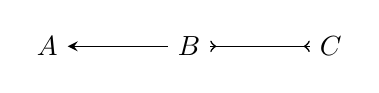
\begin{tikzpicture}[->,>=stealth,font=\sffamily,semithick,node distance=1.8cm]
		\node (A)  {$A$};
		\node (B) [right of=A]  {$B$};
		\node (C) [right of=B]  {$C$};
		\path (B) edge  node {} (A)
		(B) edge [->,>=to reversed,font=\sffamily,semithick] node {} (C)
		(C) edge [->,>=to reversed,font=\sffamily,semithick] node {} (B);
		
		\end{tikzpicture}
	}
	\caption{Examples of Reo models}
\label{fig:reoModels}
\end{figure*}

The next definition maps each canonical connector that composes a Reo model to a \relo\ program. The left hand side of each mapping rule in Definition~\ref{def:parseBaseCases} is the atomic Reo connector, while the right hand size is the resulting \relo\ atomic program $\pi_i = (f_i,b_i)$, with the same behaviour as of the Reo connector. % This will be further explored in Definition~\ref{def:parse}, an auxiliary function that interprets a Reo program $\Pi = (f,b)$ and dismembers it in an ordered sequence of connectors to be evaluated $s$, which will later be used to process an input $t$ for $\pi$.

\begin{definition}[$parse$ base cases] \label{def:parseBaseCases} Each canonical Reo connector is mapped to a \relo\ program in $parse$:% as follows:
\begin{itemize}[noitemsep]
	\item \scalebox{.8}{$\begin{tikzpicture}[->,>=stealth',font=\sffamily,semithick,node distance=1.6cm]
	\node (A) {$A$};
	\node (B) [right of=A]  {$B$};
	\path (A) edge  node {} (B);	
	\end{tikzpicture}$} to $A \to B$
	
	\item \scalebox{.8}{$\begin{tikzpicture}[->,>=stealth',font=\sffamily,semithick,node distance=1.6cm,dashed]
	\node (A)  {$A$};
	\node (B) [right of=A]  {$B$};
	\path (A) edge  node {} (B);
	\end{tikzpicture}$} to $(A,A \to B)$

	\item \scalebox{.8}{$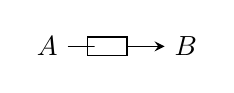
\begin{tikzpicture}[->,>=stealth,font=\sffamily,semithick,node distance=1cm]
		\node (A)  {$A$};
		\node (x) [draw,rectangle,minimum width=0.5cm,minimum height=0.2cm] at  (.76,0) {};
		\node (B) [right of=x]  {$B$};
		\draw[semithick,-] (A) -- ++(.6cm,0) |- (.4,0);
		\draw [semithick,->](x) edge  node {} (B);
		\end{tikzpicture}$} to $fifo(A,B)$
	
	\item \scalebox{.8}{$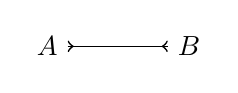
\begin{tikzpicture}[->,>=to reversed,font=\sffamily,semithick,node distance=1.8cm]
		\node (A)  {$A$};
		\node (B) [right of=A]  {$B$};% 2cm below, 1cm to the left (optional)
		\path (A) edge  node {} (B)
		(B) edge  node {} (A);
		\end{tikzpicture}$} to $SBlock(A,B)$
	
	\item \scalebox{.8}{$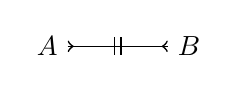
\begin{tikzpicture}[->,>=to reversed,font=\sffamily,semithick,node distance=1.8cm]
		\node (A)  {$A$};
		\node (B) [right of=A]  {$B$};
		\path (A) edge  node {\tikz \draw[|-|,semithick ] (0,0) -- +(.1,0);} (B)
		(B) edge  node {} (A);
		\end{tikzpicture}$} to $ABlock(A,B)$
	
	\item \scalebox{.8}{$\begin{tikzpicture}[->,>=stealth,font=\sffamily,semithick,node distance=1.8cm,] 
		\node (A)  {$A$};
		\node (B) [right of=A]  {$B$};% 2cm below, 1cm to the left (optional)
		\path (A) edge node {\tikz \draw[-triangle 90] (0,0) -- +(.1,0);} (B);
		\end{tikzpicture}$} to $Transform(f,A,B)$, $f \colon Data \to Data$ is a transformation function.
	
	\item \scalebox{.8}{$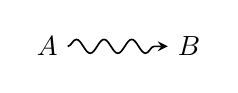
\begin{tikzpicture}[->,decorate,decoration=snake,>=stealth,font=\sffamily,semithick,node distance=1.8cm]
		\node (A)  {$A$};
		\node (B) [right of=A]  {$B$};% 2cm below, 1cm to the left (optional)
		%\path (A) edge  node (B);%{\tikz \draw [->,decorate,decoration=snake] (0,0) -- +(.1,0);} (B);
		\draw [->,decorate,decoration=snake] (A) -- (B);
		\end{tikzpicture}$} to $Filter(P,A,B)$, $P$ is a logical predicate over the data item in $A$.
	
	\item \scalebox{.8}{$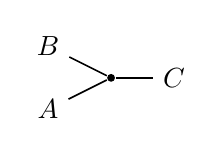
\begin{tikzpicture}[>=stealth,font=\sffamily,semithick,node distance=.8cm]
		\node (A) at (0,0) {$A$};
		\node (B) at (0,0.8)  {$B$};
		\node (x) [fill,circle,inner sep=1pt] at (0.8,0.4) {};
		\node (C) [right of=x] {$C$};
		\path (A) edge  node {} (x)
		(B) edge  node {} (x)
		(x) edge  node {} (C); %[->,thick,font=\sffamily,>=stealth] node {} (C);
		\end{tikzpicture}$} to $(A \to C, B \to C)$
	
	\item \scalebox{.8}{$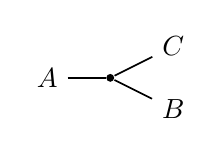
\begin{tikzpicture}[>=stealth,font=\sffamily,semithick,node distance=1cm]
		\node (A) at (0,0) {$A$} ;
		\node (x) [fill,circle,inner sep=1pt] at (0.8,0) {}; %[fill,circle,inner sep=1pt] at (0.8,0.4) {};
		\node (B) at (1.6,-0.4) {$B$};
		\node (C) at (1.6,0.4)  {$C$};
		\path (A) edge  node {} (x)
		(x) edge  node {} (B)
		(x) edge node  {} (C);
		%(x) edge[->,thick,font=\sffamily,>=stealth] node {} (C);
		\end{tikzpicture}$} to $(A \to B, A \to C)$
\end{itemize}
\end{definition}



%ERICK: 19/07/2021 - Parágrafo alterado.
Considering that each \relo\ program $\Pi$ is the composition of programs $\pi_1 \odot \pi_2, \odot \dots \odot \pi_n, \pi_i = (f_i,b_i)$ as Reo programs, $parse$ is formalized in Definition~\ref{def:parse}. The symbol $\circ$ denote the addition of an element to $s$, the resulting set of $parse$'s processing.

\begin{definition}[$parse$ function] \label{def:parse} The function that interprets the execution of a \relo\ program is defined as $parse(f, b, s)$. We define $\varepsilon$ as an abbreviation to denote when there is no \relo\ program left to process (i.e. the base case when no program is parametrized). Its outcome is detailed as below.

\begin{itemize}[noitemsep]
	\item $s, \text{ if } f = b = \varepsilon$
	\item $ %sync
	parse(f_j,b,s \circ A \to B), \text{ if } f = \begin{tikzpicture}[->,>=stealth',font=\sffamily,semithick,node distance=1.6cm,baseline=-0.85ex]
	\node (A) {$A$};
	\node (B) [right of=A]  {$B$};
	\path (A) edge  node {} (B);	
	\end{tikzpicture} \odot f_j
	$\begin{itemize}
		\item$s \circ A \to B, \text{ if } f = \begin{tikzpicture}[->,>=stealth',font=\sffamily,semithick,node distance=1.6cm]
		\node (A) {$A$};
		\node (B) [right of=A]  {$B$};
		\path (A) edge  node {} (B);	
		\end{tikzpicture}$
	\end{itemize}
	\item$ %lossysync
	parse(f_j,b,s \circ (A,A \to B)), \text{ if } f = \begin{tikzpicture}[->,>=stealth',font=\sffamily,semithick,node distance=1.6cm,dashed]
	\node (A)  {$A$};
	\node (B) [right of=A]  {$B$};
	\path (A) edge  node {} (B);
	\end{tikzpicture} \odot f_j
	$\begin{itemize}
		\item $s \circ (A,A \to B), \text{ if } f = \begin{tikzpicture}[->,>=stealth',font=\sffamily,semithick,node distance=1.6cm,dashed]
		\node (A)  {$A$};
		\node (B) [right of=A]  {$B$};
		\path (A) edge  node {} (B);
		\end{tikzpicture}$
	\end{itemize}
	\item $ %fifo
	parse(f_j,b,s) \circ fifo(A,B), \text{ if } f = 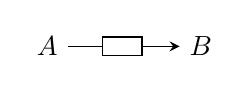
\begin{tikzpicture}[->,>=stealth,font=\sffamily,semithick,node distance=1cm]
	\node (A)  {$A$};
	\node (x) [draw,rectangle,minimum width=0.5cm,minimum height=0.2cm] at  (.95,0) {};
	\node (B) [right of=x]  {$B$};
	\draw[semithick,-] (A) -- ++(.7cm,0) |- (.5,0);
	\draw [semithick,->](x) edge  node {} (B);
	\end{tikzpicture} \odot f_j
	$\begin{itemize}
	\item $ (s \circ fifo(A,B)), \text{ if } f = 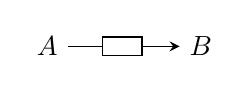
\begin{tikzpicture}[->,>=stealth,font=\sffamily,semithick,node distance=1cm]
		\node (A)  {$A$};
		\node (x) [draw,rectangle,minimum width=0.5cm,minimum height=0.2cm] at  (.95,0) {};
		\node (B) [right of=x]  {$B$};
		\draw[semithick,-] (A) -- ++(.7cm,0) |- (.5,0);
		\draw [semithick,->](x) edge  node {} (B);
		\end{tikzpicture}$
	\end{itemize}
	\item $ %syncDrain
	SBlock(A,B) \circ parse(f, b_j,s), \text{ if } b = 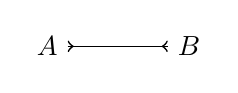
\begin{tikzpicture}[->,>=to reversed,font=\sffamily,semithick,node distance=1.8cm]
	\node (A)  {$A$};
	\node (B) [right of=A]  {$B$};% 2cm below, 1cm to the left (optional)
	\path (A) edge  node {} (B)
	(B) edge  node {} (A);
	\end{tikzpicture} \odot b_j
	$\begin{itemize}
		\item $ (SBlock(A,B) \circ s), \text{ if } b = 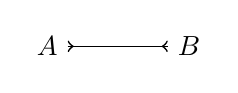
\begin{tikzpicture}[->,>=to reversed,font=\sffamily,semithick,node distance=1.8cm]
		\node (A)  {$A$};
		\node (B) [right of=A]  {$B$};% 2cm below, 1cm to the left (optional)
		\path (A) edge  node {} (B)
		(B) edge  node {} (A);
		\end{tikzpicture}$
	\end{itemize}
	\item $
	ABlock(A,B) \circ parse(f, b_j,s), \text{ if } b = 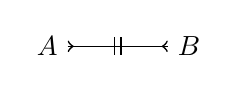
\begin{tikzpicture}[->,>=to reversed,font=\sffamily,semithick,node distance=1.8cm]
	\node (A)  {$A$};
	\node (B) [right of=A]  {$B$};
	\path (A) edge  node {\tikz \draw[|-|,semithick ] (0,0) -- +(.1,0);} (B)
	(B) edge  node {} (A);
	\end{tikzpicture} \odot b_j $
	\begin{itemize}
	\item $ (ABlock(A,B) \circ s),\text{ if } b = 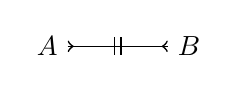
\begin{tikzpicture}[->,>=to reversed,font=\sffamily,semithick,node distance=1.8cm]
	\node (A)  {$A$};
	\node (B) [right of=A]  {$B$};
	\path (A) edge  node {\tikz \draw[|-|,semithick ] (0,0) -- +(.1,0);} (B)
	(B) edge  node {} (A);
	\end{tikzpicture}$
	\end{itemize}
	\item $ %transform
	parse(f_j,b,s \circ Transform(f,A,B)), \text{ if } f =  \begin{tikzpicture}[->,>=stealth,font=\sffamily,semithick,node distance=1.8cm,] 
	\node (A)  {$A$};
	\node (B) [right of=A]  {$B$};% 2cm below, 1cm to the left (optional)
	\path (A) edge node {\tikz \draw[-triangle 90] (0,0) -- +(.1,0);} (B);
	\end{tikzpicture} \odot f_j$
	\begin{itemize}
	\item $ (Transform(f,A,B) \circ s), \text{ if } f =  \begin{tikzpicture}[->,>=stealth,font=\sffamily,semithick,node distance=1.8cm,] 
	\node (A)  {$A$};
	\node (B) [right of=A]  {$B$};% 2cm below, 1cm to the left (optional)
	\path (A) edge node {\tikz \draw[-triangle 90] (0,0) -- +(.1,0);} (B);
	\end{tikzpicture}$ 
	\end{itemize}
	\item $ %Filter
	parse(f_j,b,s \circ Filter(P,A,B)), \text{ if } f = 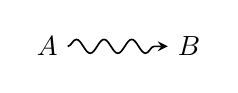
\begin{tikzpicture}[->,decorate,decoration=snake,>=stealth,font=\sffamily,semithick,node distance=1.8cm]
	\node (A)  {$A$};
	\node (B) [right of=A]  {$B$};% 2cm below, 1cm to the left (optional)
	%\path (A) edge  node (B);%{\tikz \draw [->,decorate,decoration=snake] (0,0) -- +(.1,0);} (B);
	\draw [->,decorate,decoration=snake] (A) -- (B);
	\end{tikzpicture} \odot f_j $
	\begin{itemize}
	\item $ (Filter(P,A,B) \circ s), \text{ if } f = 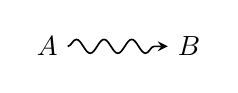
\begin{tikzpicture}[->,decorate,decoration=snake,>=stealth,font=\sffamily,semithick,node distance=1.8cm]
	\node (A)  {$A$};
	\node (B) [right of=A]  {$B$};% 2cm below, 1cm to the left (optional)
	\draw [->,decorate,decoration=snake] (A) -- (B);
	\end{tikzpicture}$
	\end{itemize}
	\item $ %merger
	parse(f_j,b,s\circ (A \to C, B \to C)), \text{ if } f = 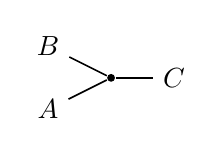
\begin{tikzpicture}[>=stealth,font=\sffamily,semithick,node distance=.8cm, baseline=0.5mm]
	\node (A) at (0,0) {$A$};
	\node (B) at (0,0.8)  {$B$};
	\node (x) [fill,circle,inner sep=1pt] at (0.8,0.4) {};
	\node (C) [right of=x] {$C$};
	\path (A) edge  node {} (x)
	(B) edge  node {} (x)
	(x) edge  node {} (C); %[->,thick,font=\sffamily,>=stealth] node {} (C);
	\end{tikzpicture} \odot f_j$
	\begin{itemize}
	\item $ (s \circ (A \to C, B \to C)), \text{ if } f = 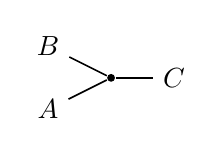
\begin{tikzpicture}[>=stealth,font=\sffamily,semithick,node distance=.8cm, baseline=0.5mm]
	\node (A) at (0,0) {$A$};
	\node (B) at (0,0.8)  {$B$};
	\node (x) [fill,circle,inner sep=1pt] at (0.8,0.4) {};
	\node (C) [right of=x] {$C$};
	\path (A) edge  node {} (x)
	(B) edge  node {} (x)
	(x) edge  node {} (C); %[->,thick,font=\sffamily,>=stealth] node {} (C);
	\end{tikzpicture}$
	\end{itemize}
	\item %\scriptstyle %replicator
	$parse(f_j,b,s\circ (A \to B, A \to C)), \text{ if } f = 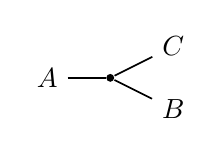
\begin{tikzpicture}[>=stealth,font=\sffamily,semithick,node distance=1cm, baseline=0.3mm]
	\node (A) at (0,0) {$A$} ;
	\node (x) [fill,circle,inner sep=1pt] at (0.8,0) {}; %[fill,circle,inner sep=1pt] at (0.8,0.4) {};
	\node (B) at (1.6,-0.4) {$B$};
	\node (C) at (1.6,0.4)  {$C$};
	\path (A) edge  node {} (x)
	(x) edge  node {} (B)
	(x) edge node  {} (C);
	%(x) edge[->,thick,font=\sffamily,>=stealth] node {} (C);
	\end{tikzpicture} \odot f_j$
	\begin{itemize}
	\item $ (s \circ (a \to b, a \to c)), \text{ if } f = 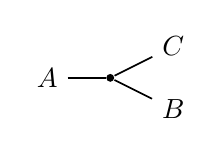
\begin{tikzpicture}[>=stealth,font=\sffamily,semithick,node distance=1cm, baseline=0.3mm]
	\node (A) at (0,0) {$A$} ;
	\node (x) [fill,circle,inner sep=1pt] at (0.8,0) {}; %[fill,circle,inner sep=1pt] at (0.8,0.4) {};
	\node (B) at (1.6,-0.4) {$B$};
	\node (C) at (1.6,0.4)  {$C$};
	\path (A) edge  node {} (x)
	(x) edge  node {} (B)
	(x) edge node  {} (C); \end{tikzpicture}$
	\end{itemize}
\end{itemize}
%\begin{equation}\scriptstyle
%parse(f, b, s) = \begin{cases}\scriptstyle
%%s\text{, iff }\pi_i = \epsilon\\
%
%s, \text{ if } f = b = \varepsilon\\
%
%%sync
%\scriptstyle
%parse(f_j,b,s \circ A \to B), \text{ if } f = \begin{tikzpicture}[->,>=stealth',font=\sffamily,semithick,node distance=1.6cm,baseline=-0.1mm]
%\node (A) {$A$};
%\node (B) [right of=A]  {$B$};
%\path (A) edge  node {} (B);	
%\end{tikzpicture} \odot f_j \\
%\hspace{2.6em} s \circ A \to B, f = \begin{tikzpicture}[->,>=stealth',font=\sffamily,semithick,node distance=1.6cm]
%\node (A) {$A$};
%\node (B) [right of=A]  {$B$};
%\path (A) edge  node {} (B);	
%\end{tikzpicture}\\
%%\hspace{2.6em} s, \text{ if } f = \varepsilon\\
%
%%\hspace{2.6em} (s \circ A \to B), \text{ iff } f_i \odot f_j = \pi_i \\
%%\hspace{4.0em}  \text{ if } \exists \pi_{j} \in acc \mid sink(\pi_{j}) = B, \text{ then } g(\pi, (s \circ \pi_i)\setminus \pi_{j}) \cup  g(\pi, s)\\
%
%%lossySync
%\scriptstyle
%parse(f_j,b,s \circ (A,A \to B)), \text{ if } f = \begin{tikzpicture}[->,>=stealth',font=\sffamily,semithick,node distance=1.6cm,dashed]
%\node (A)  {$A$};
%\node (B) [right of=A]  {$B$};
%\path (A) edge  node {} (B);
%\end{tikzpicture} \odot f_j \\
%\hspace{2.6em} s \circ (A,A \to B), f = \begin{tikzpicture}[->,>=stealth',font=\sffamily,semithick,node distance=1.6cm,dashed]
%\node (A)  {$A$};
%\node (B) [right of=A]  {$B$};
%\path (A) edge  node {} (B);
%\end{tikzpicture}\\
%%\hspace{2.6em} s, \text{ if } f = \varepsilon\\
%%\hspace{2.6em} (s \circ (a,a \to b)), \text{ iff } f_i \odot f_j = \pi_i \\
%
%
%%fifo
%\scriptstyle
%parse(f_j,b,s) \circ fifo(A,B), \text{ if } f = \begin{tikzpicture}[->,>=stealth,font=\sffamily,semithick,node distance=1cm]
%\node (A)  {$A$};
%\node (x) [draw,rectangle,minimum width=0.5cm,minimum height=0.2cm] at  (.95,0) {};
%\node (B) [right of=x]  {$B$};
%\draw[semithick,-] (A) -- ++(.7cm,0) |- (.5,0);
%\draw [semithick,->](x) edge  node {} (B);
%\end{tikzpicture} \odot f_j\\
%\hspace{2.6em} (s \circ fifo(A,B)),  f = \begin{tikzpicture}[->,>=stealth,font=\sffamily,semithick,node distance=1cm]
%\node (A)  {$A$};
%\node (x) [draw,rectangle,minimum width=0.5cm,minimum height=0.2cm] at  (.95,0) {};
%\node (B) [right of=x]  {$B$};
%\draw[semithick,-] (A) -- ++(.7cm,0) |- (.5,0);
%\draw [semithick,->](x) edge  node {} (B);
%\end{tikzpicture}\\
%
%%syncDrain
%\scriptstyle
%SBlock(A,B) \circ parse(f, b_j,s), \text{ if } b = \begin{tikzpicture}[->,>=to reversed,font=\sffamily,semithick,node distance=1.8cm]
%\node (A)  {$A$};
%\node (B) [right of=A]  {$B$};% 2cm below, 1cm to the left (optional)
%\path (A) edge  node {} (B)
%(B) edge  node {} (A);
%\end{tikzpicture} \odot b_j\\
%\hspace{2.6em} (SBlock(A,B) \circ s), b = \begin{tikzpicture}[->,>=to reversed,font=\sffamily,semithick,node distance=1.8cm]
%\node (A)  {$A$};
%\node (B) [right of=A]  {$B$};% 2cm below, 1cm to the left (optional)
%\path (A) edge  node {} (B)
%(B) edge  node {} (A);
%\end{tikzpicture}\\
%
%%\hspace{2.6em} SBlock(A,B), \text{ if } f_i \odot f_j, b_j = \emptyset\\
%%\hspace{2.6em} (SBlock(A,B) \circ s), \text{ iff } f_i \odot f_j = \pi_i \\
%
%
%%AsyncDrain
%\scriptstyle
%ABlock(A,B) \circ parse(f, b_j,s), \text{ if } b = \begin{tikzpicture}[->,>=to reversed,font=\sffamily,semithick,node distance=1.8cm]
%\node (A)  {$A$};
%\node (B) [right of=A]  {$B$};
%\path (A) edge  node {\tikz \draw[|-|,semithick ] (0,0) -- +(.1,0);} (B)
%(B) edge  node {} (A);
%\end{tikzpicture} \odot b_j\\
%\hspace{2.6em} (ABlock(A,B) \circ s), b = \begin{tikzpicture}[->,>=to reversed,font=\sffamily,semithick,node distance=1.8cm]
%\node (A)  {$A$};
%\node (B) [right of=A]  {$B$};
%\path (A) edge  node {\tikz \draw[|-|,semithick ] (0,0) -- +(.1,0);} (B)
%(B) edge  node {} (A);
%\end{tikzpicture}\\
%%\hspace{2.6em} ABlock(A,B), \text{ if } f_i \odot f_j, b_j = \emptyset\\
%
%
%%transform
%\scriptstyle
%parse(f_j,b,s \circ Transform(f,A,B)), \text{ if } f =  \begin{tikzpicture}[->,>=stealth,font=\sffamily,semithick,node distance=1.8cm,] 
%\node (A)  {$A$};
%\node (B) [right of=A]  {$B$};% 2cm below, 1cm to the left (optional)
%\path (A) edge node {\tikz \draw[-triangle 90] (0,0) -- +(.1,0);} (B);
%\end{tikzpicture} \odot f_j\\
%\hspace{2.6em} (Transform(f,A,B) \circ s), f =  \begin{tikzpicture}[->,>=stealth,font=\sffamily,semithick,node distance=1.8cm,] 
%\node (A)  {$A$};
%\node (B) [right of=A]  {$B$};% 2cm below, 1cm to the left (optional)
%\path (A) edge node {\tikz \draw[-triangle 90] (0,0) -- +(.1,0);} (B);
%\end{tikzpicture}\\
%%\hspace{2.6em} Transform(f,A,B), \text{ if } f_j, b_i \odot b_j = \emptyset\\
%%\hspace{2.6em} (Transform(f,A,B) \circ s), \text{ iff } f_i \odot f_j = \pi_i \\
%
%%filter
%\scriptstyle
%parse(f_j,b,s \circ Filter(P,A,B)), \text{ if } f = \begin{tikzpicture}[->,decorate,decoration=snake,>=stealth,font=\sffamily,semithick,node distance=1.8cm]
%\node (A)  {$A$};
%\node (B) [right of=A]  {$B$};% 2cm below, 1cm to the left (optional)
%%\path (A) edge  node (B);%{\tikz \draw [->,decorate,decoration=snake] (0,0) -- +(.1,0);} (B);
%\draw [->,decorate,decoration=snake] (A) -- (B);
%\end{tikzpicture} \odot f_j\\
%\hspace{2.6em} (Filter(P,A,B) \circ s), f = \begin{tikzpicture}[->,decorate,decoration=snake,>=stealth,font=\sffamily,semithick,node distance=1.8cm]
%\node (A)  {$A$};
%\node (B) [right of=A]  {$B$};% 2cm below, 1cm to the left (optional)
%%\path (A) edge  node (B);%{\tikz \draw [->,decorate,decoration=snake] (0,0) -- +(.1,0);} (B);
%\draw [->,decorate,decoration=snake] (A) -- (B);
%\end{tikzpicture}\\
%%\hspace{2.6em} Filter(P,A,B), \text{ if } f_j, b_i \odot b_j = \emptyset\\
%%\hspace{2.6em} (Filter(P,A,B) \circ s), \text{ iff } f_i \odot f_j = \pi_i \\
%
%%merger
%\scriptstyle
%parse(f_j,b_i \odot b_j,s\circ (A \to C, B \to C)), \text{ if } f = \begin{tikzpicture}[>=stealth,font=\sffamily,semithick,node distance=.8cm, baseline=0.5mm]
%\node (A) at (0,0) {$A$};
%\node (B) at (0,0.8)  {$B$};
%\node (x) [fill,circle,inner sep=1pt] at (0.8,0.4) {};
%\node (C) [right of=x] {$C$};
%\path (A) edge  node {} (x)
%(B) edge  node {} (x)
%(x) edge  node {} (C); %[->,thick,font=\sffamily,>=stealth] node {} (C);
%\end{tikzpicture} \odot f_j\\
%\hspace{2.6em} (s \circ (A \to C, B \to C)), f = \begin{tikzpicture}[>=stealth,font=\sffamily,semithick,node distance=.8cm, baseline=0.5mm]
%\node (A) at (0,0) {$A$};
%\node (B) at (0,0.8)  {$B$};
%\node (x) [fill,circle,inner sep=1pt] at (0.8,0.4) {};
%\node (C) [right of=x] {$C$};
%\path (A) edge  node {} (x)
%(B) edge  node {} (x)
%(x) edge  node {} (C); %[->,thick,font=\sffamily,>=stealth] node {} (C);
%\end{tikzpicture} \\
%%\hspace{2.6em} (A \to C, B \to C), \text{ if } f_j, b_i \odot b_j = \emptyset\\
%%\hspace{2.6em} (s \circ (a \to c, b \to c)), \text{ iff } f_i \odot f_j = \pi_i \\
%
%%Replicator
%\scriptstyle
%parse(f_j,b,s\circ (A \to B, A \to C)), \text{ if } f = \begin{tikzpicture}[>=stealth,font=\sffamily,semithick,node distance=1cm, baseline=0.3mm]
%\node (A) at (0,0) {$A$} ;
%\node (x) [fill,circle,inner sep=1pt] at (0.8,0) {}; %[fill,circle,inner sep=1pt] at (0.8,0.4) {};
%\node (B) at (1.6,-0.4) {$B$};
%\node (C) at (1.6,0.4)  {$C$};
%\path (A) edge  node {} (x)
%(x) edge  node {} (B)
%(x) edge node  {} (C);
%%(x) edge[->,thick,font=\sffamily,>=stealth] node {} (C);
%\end{tikzpicture} \odot f_j\\
%\hspace{2.6em} (s \circ (a \to b, a \to c)), f = \begin{tikzpicture}[>=stealth,font=\sffamily,semithick,node distance=1cm, baseline=0.3mm]
%\node (A) at (0,0) {$A$} ;
%\node (x) [fill,circle,inner sep=1pt] at (0.8,0) {}; %[fill,circle,inner sep=1pt] at (0.8,0.4) {};
%\node (B) at (1.6,-0.4) {$B$};
%\node (C) at (1.6,0.4)  {$C$};
%\path (A) edge  node {} (x)
%(x) edge  node {} (B)
%(x) edge node  {} (C);
%%(x) edge[->,thick,font=\sffamily,>=stealth] node {} (C);
%\end{tikzpicture}\\
%%\hspace{2.6em} (A \to B, A \to C), \text{ if } f_j, b_i \odot b_j = \emptyset\\
%%\hspace{2.6em} (s \circ (a \to b, a \to c)), \text{ iff } f_i \odot f_j = \pi_i \\
%\end{cases}
%\end{equation}
\end{definition}

%erick: parágrafo explicando os programas de parse embutido no parágrafo abaixo:]
We employ $parse$ to interpret Reo programs $\Pi$ as a sequence of occurrences of possible data flow (where each flow corresponds to the execution of a Reo connector). These data flow may denote data transfer (\relo\ programs ($A \to B$) and ($A$,$A \to B$), flow ``blocks'' induced by connectors such as SyncDrain and aSyncDrain (\relo\ programs $SBlock(A,B)$ and $ABlock(A,B)$ --- the first one requires that data flow synchronously through its ports, while the latter requires that data flow asynchronously through its ports). There is also the notion of a buffer introduced by FIFO connectors (\relo\ program $fifo(A,B)$), which data flow into a buffer before flowing out of the channel, and merging/replicating data flow between ports, respectively denoted by channels Merger and Replicator (\relo\ programs $(A \to C, B \to C)$ and $(A \to B, A \to C)$ respectively). 

There are also special data flows, denoting the ``transformation'' of some data flowing from A to B as $Transform(f,A,B)$ which will apply $f$ with the data in $A$ before it sends $f(D_A)$ ($D_A$ denoting the data item in A) to $B$, and the filtering of data flow by some predicate as $Filter(P,A,B)$, $P$ as a quantifiable-free predicate over the data item seen in $A$. Therefore, data will flow to $B$ only if $P(D_A)$ is satisfied.

After processing $\pi$ with $parse$, the interpretation of the execution of $\pi$ is given by $go(t,s,acc), go\colon s \times s \to s$, where $s$ is a string denoting the processed program $\pi$ as the one returned by $parse$, and $t$ is the initial data flow of ports of the Reo program $\pi$. The parameter $acc$ holds all connectors of the Reo circuit that satisfy their respective required conditions for data to flow. In what follows we define $ax \prec t$ as an operator which states that $ax$ is in $t$, $ax$ a single data of a port and $t$ a structure containing data flows for ports $p \in \mathcal{N}$.

Example~\ref{def:gExample} shows how $parse$ functions and illustrates why it is necessary. The programs that depict the FIFO connectors from Fig.~\ref{fig:SequencerReo} are the last programs to be executed, while the ones that denote ``immediate'' flow (the Sync channels) come first. This is done to preserve the data when these connectors fire (if eligible). Suppose that there is a data item in the buffer between X and Y and a data item in Y (i.e., $t = X1Y, Y0$). If the data item leaves the buffer first then the data item in Y, the latter will be overwritten and the information is lost.

\begin{example} \label{def:gExample}
	let $\pi$ be the Reo program corresponding to the circuit in Fig.~\ref{fig:SequencerReo}:\\
	$\pi$ = \scalebox{0.7}[0.7]{ $\rfifo{X}{Y} \odot \rsync{Y}{A} \odot \rfifo{Y}{W} \odot \rsync{W}{B} \odot \rfifo{W}{Z} $}\\ \scalebox{0.7}[0.7]{ $\odot \rsync{Z}{C} \odot \rsync{Z}{X}$}\\
	$parse(\pi,\{\})$ = \{$Y \to A; W \to B ; Z \to C ; Z \to X ; fifo(X,Y); fifo(Y,W);fifo(W,Z)$\}
\end{example}

The usage of $parse$ is required to eliminate problems regarding the execution order of $\pi$'s Reo channels, which could be caused by processing $\pi$ the way it is inputted (i.e., its connectors can be in any order). Consider, for example, the behavior of SyncDrain and aSyncDrain programs as ``blocking'' programs as discussed earlier. In a single step, they must be evaluated before the flow programs, because if they fail to execute due to missing requirements, data should not flow from their port names to other connectors. In a nutshell, $parse$ organizes the program so this verification can be performed.

Therefore, the interpretation of a $\pi$ program processed by $parse$ is performed by $go(t,s,acc)$, where $s$ is a string containing $\pi$ as processed by $parse$, $t$ is $\pi$'s initial data flow, and $acc$ filters the connectors of the \relo\ program that can be fired if the requirements to do so are met.

%ERICK: 19/07/2021 - Parágrafo adicionado.
Definition \ref{def:go} will check for each of the Reo connectors processed by $parse$ satisfies the required condition to fire, following the connectors' behaviour. Operator $\prec$ denotes whether the data flow is within the current data flow $t$ being evaluated. It is also used to denote whether the program currently being evaluated in $s$ repeats in $\Pi$. Operator $\setminus$ denotes the removal of an connector from the accumulator $acc$.
%\newpage

\begin{definition}[Relation $go$ for a single execution step] \label{def:go} We define $go(t,s,acc)$ as follows:
	
	%\erick{21/11 - adicionada clausula do $\epsilon$, othwerwise p/ casos de erro (i.e., quando praquele cenário o conector não deve disparar). Não me parece necessário para os blocks.}
	%\erick{24/11 - Clausula $\epsilon$ interrompia o funcionamento em um primeiro conector que nao pudesse disparar. Trocada para $go(t,s',acc)$ --- chamada recursiva para o resto do programa, sem considerar o conector que ``falhou''}
	\begin{itemize}[noitemsep]
		
		\item $s = \epsilon : fire(t,acc)$
		
		%sync
		\item $s = A \to B \circ s' : $\begin{itemize}[noitemsep]
			\item $go(t,s',acc \circ (A \to B)), \text{ iff }  Ax \prec t, (A \to B) \nprec s'$ 
			\item $go(t,s', (acc \circ (A \to B))\setminus s'_{j}) \cup  go(t, s',acc), \text{ iff } \begin{cases}
			Ax \prec t,\\
			(A \to B) \nprec s' \\
			\exists s'_{j} \in acc \mid sink(s'_{j}) = B \end{cases}$
			\item $go(t,s',acc)$, otherwise
		\end{itemize}
		
		%LossySync
		\item $s = (A,A \to B) \circ s' : $\begin{itemize}[noitemsep]
			\item $go(t,s',acc \circ (A \to B)) \cup go(t,s',acc \circ (A \to A)) , \text{ iff }  Ax \prec t, (A \to B) \nprec s'$ 
			\item $go(t,s', (acc \circ (A \to B))\setminus s'_{j}) \cup  go(t, s',acc), \text{ iff } \begin{cases}
			Ax \prec t,\\
			(A \to B) \nprec s' \\
			\exists s'_{j} \in acc \mid sink(s'_{j}) = B \end{cases}$
			\item $go(t,s',acc)$, otherwise
		\end{itemize}
		
		%fifo : duas interpretações:
		%erick: 07/11 - acc \circ (axb) ou acc \circ (fifo(a,b))
		\item $s = fifo(A,B) \circ s' :$
		\begin{itemize}[noitemsep]
			
			%a) leio de s um fifo(a,b) obs: aqui, s' só tem fifos
			\item $go(t,s',acc \circ (AxB)), \text{ iff } Ax \prec t, fifo(A,B) \nprec s',(AxB) \nprec acc$
			
			%b) leio o dado que estava armazenado no fifo (axb \prec t), indica que em algum momentoe entrou dado
			\item $go(t,s', acc \circ (AxB \to Bx)), \text{ iff } AxB \prec t, fifo(A,B) \nprec s'$
			
			%c): alguém que tenha o mesmo destino do fifo já foi processado e pode disparar, nesse caso precisamos de execuções não deterministicas. Note que isso só afeta a execução de quando o dado é lido do buffer para a porta destino.
			\item $go(t,s',(acc \circ (AxB \to Bx) )\setminus s'_{j}) \cup  go(t, s',acc), \text{ iff } \begin{cases} AxB \prec t,\\ fifo(A,B) \nprec s',\\ \exists s'_{j} \in acc \mid sink(s'_{j}) = B\\\end{cases}$ 
			\item $go(t,s',acc)$, otherwise
		\end{itemize}
		
		%SyncDrain
		\item 	$s = Sblock(A,B) \circ s' :$ \begin{itemize}[noitemsep]
			%tres casos:
			%a) caso o comportamento esperado seja atingido: dados em ambas as portas ou em nenhuma
			\item $go(t,s',acc), \text{ iff } \begin{cases}  (Ax \prec t \land Bx \prec t) \lor (Ax \nprec t \land Bx \nprec t) \\ Sblock(A,B) \nprec s' \end{cases}$ 
			%b) caso apenas uma das portas tenha dados: retirar de s qualquer passagem de dado que envolve as portas do drain corrente
			\item $go(t,halt(A,B,s'),acc), \text{ iff } \begin{cases} (Ax \prec t \land Bx \nprec t) \lor (Ax \nprec t \land Bx \prec t)\\  Sblock(A,B) \nprec s' \end{cases}$
			%erick: 16/11 c) caso não determinístco (vale para ambos os nós do conector) --- pensar 
		\end{itemize}
		
		%AsyncDrain
		\item $s = Ablock(A,b)\circ s':$
		%dois casos:
		%a) caso o comportamento esperado seja atingido: dados em ambas as portas ou em nenhuma
		\begin{itemize}[noitemsep]
			\item $go(t,s',acc), \text{ iff } \begin{cases} (Ax \nprec t \land Bx \prec t) \lor (Ax \prec t \land Bx \nprec t) \lor \\ (Ax \nprec t \land Bx \nprec t), Ablock(A,B) \nprec s'\end{cases}$ 
			%b) caso as duas portas possuam dados simultaneamente: retirar de s qualquer passagem de dado que envolve as portas do drain corrente
			\item $go(t,halt(A,B,s'),acc), \text{ iff } \begin{cases} (Ax \prec t \land Bx \prec t), \\  Ablock(A,B) \nprec s' \end{cases}$
			%erick: 16/11 - Nao determinismo tal como para o syncDrain acima. pensar
		\end{itemize}
		
		%Transformer 
		\item $s = Transform(f,A,B) \circ s' : $\begin{itemize}[noitemsep]
			\item $go(t,s',acc \circ (f(D_A) \to B)), \text{ iff }\begin{cases} 
			ax \prec t\\ 
			Transform(f,A,B) \nprec s' \end{cases}$ 
			\item $go(t,s', (acc \circ (f(D_A) \to B))\setminus s'_{j}) \cup  go(t, s',acc), \text{ iff } \begin{cases}
			Ax \prec t,\\
			Transform(f,A,B) \nprec s' \\
			\exists s'_{j} \in acc \mid sink(s'_{j}) = B \end{cases}$
			\item $go(t,s',acc)$, otherwise
		\end{itemize}
		
		%Filter 
		\item $s = Filter(f,A,B) \circ s' : $\begin{itemize}[noitemsep]
			\item $go(t,s',acc \circ (A \to B)), \text{ iff }\begin{cases} 
			Ax \prec t\\ 
			P(D_A) \text{ holds }\\
			Filter(f,A,B) \nprec s' \end{cases}$ 
			\item $go(t,s', (acc \circ (A \to B))\setminus s'_{j}) \cup  go(t, s',acc), \text{ iff } \begin{cases}
			Ax \prec t,\\
			P(D_A) \text{ holds }\\
			Filter(f,A,B) \nprec s' \\
			\exists s'_{j} \in acc \mid sink(s'_{j}) = B \end{cases}$
			\item $go(t,s',acc)$, otherwise
		\end{itemize}
		
		%%merger
		%\item $s = (a \to c, b \to c)\circ s' :$
		%	\begin{itemize}[noitemsep]
		%	%erick: 16/11 - rever isso aqui. eu escrevi o replicator no lugar do merge
		%	\item $go(t,s', acc \circ (a \to c)) \cup go(t,s', acc \circ (b \to c))), \text{ iff } \begin{cases} ax  \prec t, by \nprec t\\ (a \to b, a \to c) \nprec s' \end{cases}$
		%	%nao determinismo: uma execucao com cada perna do merger mais o que já estava lá (3 no total)
		%	\item $go(t,s',acc \circ (a \to c) \setminus s'_j) \cup go(t,s',acc \circ (b \to c) \setminus s'_j) \cup go(t,s',acc) , \text{ iff } \begin{cases} ax  \prec t, by \nprec t\\ (a \to b, a \to c) \nprec s'\\ \exists s'_{j} \in acc \mid sink(s'_{j}) = c \end{cases}$
		%	\end{itemize}
		
		
		%replicator (o boladao que pus no lugar do merger) 
		%apenas 1 dos 2 ja tem um sink no acc
		%caso c seja o destino ja em acc
		%\item $go(t,s',acc \circ (a \to c) \setminus s'_j) \cup\\ go(t,s',acc \circ (a \to b)),\text{ iff }
		%\begin{cases}
		%ax \prec t,\\
		%(a \to b \to c) \nprec s',\\
		%\exists s'_{j} \in acc \mid sink(s'_{j}) = b \end{cases}$
		%
		%%caso b seja o destino ja em acc
		%\item $go(t,s',acc \circ (a \to b) \setminus s'_j) \cup\\ go(t,s',acc \circ (a \to c)), \text{ iff }
		%\begin{cases}
		%ax \prec t,\\
		%(a \to b \to c) \nprec s',\\
		%\exists s'_{j} \in acc \mid sink(s'_{j}) = c \end{cases}$
		%
		%%ambas as portas tem o sink em acc
		%\item $go(t,s',acc \circ (a \to b) \setminus s'_j) \cup\\ go(t,s',acc \circ (a \to c) \setminus s'k),\text{ iff }
		%\begin{cases}
		%ax \prec t,\\
		%(a \to b \to c) \nprec s',\\
		%\exists s'_{j} \in acc \mid sink(s'_{j}) = b,\\
		%\exists s'_{k} \in acc \mid sink(s'_{k}) = c,
		%\end{cases}$
		
	\end{itemize}
\end{definition}

The existing condition after each return condition of $go$ denotes the case where two or more Reo connectors within a circuit have the same sink node. This implies that if both of their respective source nodes have data flowing simultaneously, their sink nodes will have data flowing nondeterministically. Such condition models this scenario, considering when both cases may happen as two nondeterministic ``distinct'' possible executions. Therefore, the operation $acc \circ (X \to Y))\setminus s'_{j}$ removes every interpretation of $s'$ which sink node equals $Y$, while $go(t, s',acc)$ denotes an execution containing the removed $s'_{j}$ but not considering $X \to Y$. The return condition $s = \epsilon$ denotes that the program as a whole has already been processed.

Considering the cases including block programs induced by SyncDrain and AsyncDrain connectors, $halt(A,B,s')$ is defined as a supporting function that will be used in the case the block program conditions fail. Then, data flow that was in the ports of the SyncDrain/AsyncDrain evaluated cannot be further considered in this execution steps: channels that have their sink node pointed to $A$ or $B$.

Intuitively, $go$ is a function that processes a program $\pi$ with input $t$ as the program's data initially available at ports $p \in \pi$ and returns the next data configuration after processing all connectors and verifying whether they are eligible for data to flow. The return of $go$ depends on a function $fire$ which is bound to return the final configuration of the Reo circuit after an iteration (i.e., the last ports that data flow). We define $sink(s'_j)$ as the sink node of a connector, in this case, the port name where a data item flowing into a Reo connector is bound to. The operation denoted by $\cup$ is the standard set union.

%ERICK - 19/07/2021 - Parágrafo abaixo reescrito
Definition $go$ employs a function named $fire\colon T \times s \rightarrow T$ which returns the firing of all possible data flows in the Reo connector, given the Reo program $\pi$ and an initial data flow on ports of $\pi$. The set $T$ is the set of possible data flows as constructed by the BNF grammar in Definition~\ref{def:reloLanguage}. The function $fire$ returns the resulting data flow of this execution step by considering the program processed by $go$ as $s$ and the current step's data flow $t$. Parameter $s$ contains \relo\ programs as yielded by $parse$.

\begin{definition}[Data marking relation $fire$] \label{def:fire}
%erick:11/11 - modificação em fire para refletir o disparo "simples" (por iteração) nos conectores:
%modificações:
%1) \nexists c \mid (b \to c) \prec s \text{ and } bx \prec t\\ %erick: 07/11 - else fire(t,s')? => \text{ if } s = (a \to b) \circ s' \text{ and } ax \prec t\\
%2)  axb \prec t =>  ax \prec t 

%\erick{11/11 - não sei se fire é necessária. Como nosso disparo é ``passo a passo'' (uma iteração de cada vez), me parece que o resultado dos disparos podem ser acumulados no próprio acc, ao inves das referências de disparos (uma vez que nesse cenário, t não é modificada, mantendo apenas as marcações iniciais).}\\
%\erick{12/11 - me parece sim ser necessária.Um exemplo: go se livra de blocks (se possível), e fire apenas recebe uma sequênciac orreta e dispara. Creio que essa divisão nos facilitará a definição de modelo, inclusive}
%\bruno{Sim, é necessário para a definição do modelo.}


\begin{align}
fire(t,s) = \begin{cases}
%se não tem sequência pra executar, não executo
\epsilon, \text{ if } s = \epsilon \\
%disparo normal
%bx \circ fire(t,s'), \text{ if } s = (a \to b) \circ s' \text{ and } ax \prec t\\ %erick: 10/03 - reorganização da escrta - clausula unificada com o bx la embaixo 
%dado entra no fifo
AxB \circ fire(t,s'), \text{ if } s = (AxB) \circ s' \text{ and } Ax \prec t\\
%dado de transformer
B(f(a)) \circ fire(t,s'), \text{ if } s = (f(D_A) \to B) \circ s' \text{ and } Ax \prec t\\
Bx \circ fire(t,s'), \text{ if } \begin{cases} 
%disparo normal
s = (A \to B) \circ s' \text{ and } Ax \prec t, or\\
%dado sai no fifo
s = (AxB \to Bx) \circ s' \text{ and } axb \prec t\\
\end{cases}\\
\end{cases}
\end{align}

\end{definition}

We define $f_{ReLo}$ as the transition relation of a \relo\ model. It denotes how the transitions of the model fire, i.e., given an input $t$ and a program $\pi$ denoting a Reo circuit, $f_{ReLo}(t,\pi)$ interfaces with $go$ to return the resulting data flow of $\pi$ given that data depicted by $t$ are flowing in the connector's ports.

\begin{definition}{Transition relation} \label{def:f}
%\bruno{Precisamos definir um símbolo para sequência vazia.}
%\erick{$\epsilon?$ Para mim, $\epsilon$ pode significar tanto quando seuqncia é vazia quanto um programa $\pi$ vazio (vide as definições $parse$ e $go$). Pus na seção 1} -> edit: 19/04 - não existe programa vazio. logo, epsilon denota a sequencia vazia.
$f_{ReLo}(t,\pi) = go(t,(parse(\pi,[])),[])$

\end{definition}

We define $f_{ReLo}(t,\pi^\star)$ as the application of $f_{ReLo}(t,\pi)$ iteratively for the (nondeterministic finite) number of steps denoted by $\star$, starting with $t$ with $\pi$, and considering the obtained intermediate $t'$ in the steps.%ERICK: 18/07/2021 - Inserido após colocar a definição t_(f,b^\star) no axioma ind.

A \relo\ frame is a structure based on Kripke frames~\cite{Kripke1959} formally defined as a tuple $\mathcal{F} = \langle S, \Pi ,R_\Pi, \delta,$ $\lambda \rangle$, where each element of $\mathcal{F}$ is described by Definition~\ref{def:reloFrame}.

\begin{definition}[\relo\ frame] \label{def:reloFrame}  $S$ is a non-empty enumerable set of states and $\Pi$ a Reo program.
	\begin{itemize}[noitemsep]
		\item $R_\Pi \subseteq S \times S$ is a relation defined as follows.
		\begin{itemize}[noitemsep]
			\item $R_{\pi_i} =	\lbrace uR_{\pi_i}v \mid f_{ReLo}(t,\pi_i) \prec \delta(v)$, $t \prec \delta(u) \rbrace$, $\pi_i$ is any combination of any atomic program which is a subprogram of $\Pi$.%\erick{e agora?}% <--- $\forall\pi_i\propto\Pi$}
			\item $R_{\pi_i^\star} = R^\star_{\pi_i}$, the reflexive transitive closure (RTC) of $R_{\pi_i}$.	
		\end{itemize}
		%erick: texto removido do item do pi -> \bruno{describing how a Reo circuit (denoted by program $\pi$) changes its configuration (i.e., how data flow through the connector), where each state denote a specific data flow the connector may describe. $R_\Pi$ is described by means of each subprogram of $\Pi$ --> remover} \bruno{algo na forma $\forall\pi_i\propto\Pi$}. 
		\item $\lambda \colon S \times \mathcal{N} \rightarrow \mathbbm{R}$ is a function that returns the time instant a data item in a data markup flows through a port name of $\mathcal{N}$.
		\item $\delta \colon S \rightarrow T$, is a function that returns data in ports of the circuit in a state $s \in S$, $T$ being the set of possible data flows in the model.
		
		
	\end{itemize}
\end{definition}

From Definition~\ref{def:reloFrame}, a \relo\ model is formally defined as a tuple $\mathcal{M} = \langle \mathcal F,  \textbf{V} \rangle$ by Definition~\ref{def:reloModels}. Intuitively, it is a tuple consisting of a \relo\ frame and a valuation function, which given a state $w$ of the model and a propositional symbol $\varphi \in \Phi$, maps to either $true$ or $false$.%, depending on the formula satisfiability on state $w$.

\begin{definition}[\relo\ models] \label{def:reloModels} A model in \relo\ is a tuple $\mathcal{M} = \langle \mathcal F,  \textbf{V} \rangle$, where $\mathcal{F}$ is a \relo\ frame and $V\colon S \times \Phi \to \{true,false\}$ is the model's valuation function
\end{definition}

%$R_\pi \subseteq S \times S$ is a binary relation over the set of states $S$, denoting how states of the model relate to each other. Intuitively, $R_\Pi$ denotes how the changing of states happens on program $\pi$ (i.e., after each firing, what has changed by the program's execution). Such changing is obtained directly by applying $go$ with the interpretation of $\Pi$ as the string $s$ which is result of processing $g(\pi,s)$, which is the firing function $f$'s definition. We therefore define $R_\Pi$ formally as an inductive relation over a Reo program $\Pi = \pi_1 \odot \pi_2 \dots \odot \pi_n$ as follows. Let $t = \delta(u)$ as the data at some $\pi_i$'s ports in state $u$, with $i \in 1,2,\dots,n$.
%
%\begin{align}
%R_\Pi =
%\lbrace uR_{\pi}v \mid f_{ReLo}(t,\pi_i) \prec \delta(v) \rbrace
%%erick: essa linha parece compreender o caso de f_{ReLo}(s,a) = \epsilon iff w = v
%\end{align}

%\subsection{Semantic notion of \relo} \label{subsec:semanticNotion}
%We define \relo's semantic notion intuitively as follows. Let $\mathcal{M} = \langle \mathcal F, \textbf{V} \rangle$ and $p, p_1$ and $p_2$ be propositional formula. The notion of satisfaction of a formula $p$ in $\mathcal{M}$ at a state $s \in S$ of the model, denoted by $\mathcal{M},s \Vdash p$ is defined as follows.

\begin{definition}[Satisfaction notion] \mbox{}
\begin{itemize}[noitemsep]
	\item $\mathcal{M}{,}s \Vdash p \text{ iff } V{(s,p)} = true$%\bruno{,\textnormal{ponha sempre a vírgula entre chaves nesses casos, pra remover o espaço posterior desnecessário}}
	\item $\mathcal{M}{,}s \Vdash \top$ always
	\item $\mathcal{M}{,}s \Vdash \neg \varphi \text{ iff } \mathcal{M},s \nVdash \varphi$
	\item $\mathcal{M}{,}s \Vdash \varphi_1 \land \varphi_2 \text{ iff } \mathcal{M}{,}s \Vdash \varphi_1$ and $\mathcal{M}{,}s \Vdash \varphi_2$
	\item $\mathcal{M}{,}s \Vdash \langle t, \pi \rangle \varphi$ if there exists a state $w \in S$, $sR_{\pi}w$, and $\mathcal{M}{,}s \Vdash \varphi$
\end{itemize}
We denote by $\mathcal M\Vdash\varphi$ if $\varphi$ is satisfied in all states of $\mathcal M$. By $\Vdash\varphi$ we denote that $\varphi$ is valid in any state of any model.
\end{definition}

%\erick{talvez seja interessante tirar esses dois parágrafos e guardar só pro usage example mesmo.}\\
We recover the circuit in Fig.~\ref{fig:SequencerReo} as an example. Let us consider s = $D_X$, (i.e. t = D1) and the Sequencer's corresponding model $\mathcal{M}$. Therefore, $\mathcal{M},D_X \Vdash \langle t, \pi \rangle p$ holds if $V(D_{XfifoY}, p) = true$ as $D_{XfifoY}$ is the only state where $D_X R_\Pi D_{XfifoY}$. For example, one might state $p$ as ``There is no port with any data flow'', hence $V(D_{XfifoY}, p) = true$.

As another usage example, we formalize some properties which may be interesting for this connector to have. Let us consider that the data markup is $t = X1$, $\mathcal{M}$ the model regarding the Sequencer, and the states' subscript denoting which part of the connector has data. The following example state that for this data flow, after every single execution of $\pi$, it is not the case that the three connected entities have their data equal to $1$ simultaneously, but it does have data in its buffer from $X$ to $Y$. 

%erick: 11/04 - segunda frase do parágrafo acima modificada: adicionada coisas sobre o modelo (quem é M e os estados que são mostrados no exemplo -> ``, $\mathcal{M}$ the model regarding the Sequencer, and the states' subscript denoting which part of the connector have data".). Além dessa modificação, alterei o final do segundo exemplo, onde da metade dele p baixo eu havia erroneamente trocado a modalidade de <> para [].

\begin{example}%\bruno{Na relação use o conector, não o elemento de $parse$.}
	
	\noindent$\lbrack X1,\pi \rbrack \neg (D_A = 1 \land D_B = 1 \land D_C = 1) \land t' = X1Y$, where $t' = f_{ReLo}(t,\pi)$\\
	$\mathcal{M}{,}D_X \Vdash \lbrack X1,\pi \rbrack \neg (D_A = 1 \land D_B = 1 \land D_C = 1) \land t' = X1Y$.\\
	$\mathcal{M}{,}D_{\scalebox{0.5}[0.5]{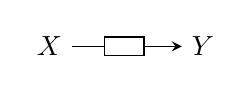
\begin{tikzpicture}[->,>=stealth,font=\sffamily,semithick,node distance=1cm]
			\node (A)  {$X$};
			\node (x) [draw,rectangle,minimum width=0.5cm,minimum height=0.2cm] at  (.95,0) {}; %[draw=black,rectangle,inner sep=5pt] at  (.88,0) {} ;
			%\node (x) [circle,fill,inner sep=1pt,right of=A] {};
			%\node (y) [circle,fill,inner sep=1pt,right of=x] {};
			\node (B) [right of=x]  {$Y$};
			\draw[semithick,-] (A) -- ++(.7cm,0) |- (.5,0);
			\draw [semithick,->](x) edge  node {} (B);
			
\end{tikzpicture}}} \Vdash  \neg (D_A = 1 \land D_B = 1 \land D_C = 1) \land t' = X1Y$.\\
$\mathcal{M}{,}D_{\scalebox{0.5}[0.5]{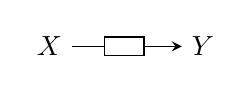
\begin{tikzpicture}[->,>=stealth,font=\sffamily,semithick,node distance=1cm]
		\node (A)  {$X$};
		\node (x) [draw,rectangle,minimum width=0.5cm,minimum height=0.2cm] at  (.95,0) {}; %[draw=black,rectangle,inner sep=5pt] at  (.88,0) {} ;
		%\node (x) [circle,fill,inner sep=1pt,right of=A] {};
		%\node (y) [circle,fill,inner sep=1pt,right of=x] {};
		\node (B) [right of=x]  {$Y$};
		\draw[semithick,-] (A) -- ++(.7cm,0) |- (.5,0);
		\draw [semithick,->](x) edge  node {} (B);
		
		\end{tikzpicture}}}
\Vdash  \neg (D_A = 1 \land D_B = 1 \land D_C = 1) \text{ and } 
\mathcal{M},D_{\scalebox{0.5}[0.5]{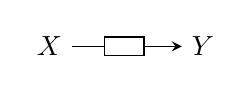
\begin{tikzpicture}[->,>=stealth,font=\sffamily,semithick,node distance=1cm]
		\node (A)  {$X$};
		\node (x) [draw,rectangle,minimum width=0.5cm,minimum height=0.2cm] at  (.95,0) {}; %[draw=black,rectangle,inner sep=5pt] at  (.88,0) {} ;
		%\node (x) [circle,fill,inner sep=1pt,right of=A] {};
		%\node (y) [circle,fill,inner sep=1pt,right of=x] {};
		\node (B) [right of=x]  {$Y$};
		\draw[semithick,-] (A) -- ++(.7cm,0) |- (.5,0);
		\draw [semithick,->](x) edge  node {} (B);
		
		\end{tikzpicture}}} \Vdash t' = X1Y$.\\


\end{example}

%Considering the scenarios where is interesting to reason regarding iteration,
The notion of $\mathcal{M},D_X \Vdash \langle t, \pi^\star \rangle p$ holds if a state $s$ is reached from $D_X$ by means of $R_\pi^\star$ with $V(s,p) = \top$. If we state $p$ as ``the data item of port $X$ equals $1$'', it holds because $D_X R_\pi^\star D_X$ and $V(D_X, p) = \top$. If there is an execution of $\pi$ that lasts a nondeterministic finite number of iterations, and there is data in $C$ equals to $1$, then there is an execution under the same circumstances where the same data has been in $B$.

\begin{example}
$\langle t,\pi^\star \rangle D_C = 1 \rightarrow \langle t, \pi^\star \rangle D_B = 1 $ \\
$\mathcal{M}{,}D_X \Vdash \langle t,\pi^\star \rangle D_C = 1 \rightarrow \langle t, \pi^\star \rangle D_B = 1 $\\
$\mathcal{M}{,}D_X \Vdash \neg( \langle t,\pi^\star \rangle D_C = 1) \lor \langle t, \pi^\star \rangle D_B = 1 $\\
$\mathcal{M}{,}D_X \Vdash \lbrack t,\pi^\star \rbrack \neg D_C = 1 \lor \langle t, \pi^\star \rangle D_B = 1 $\\
$\mathcal{M}{,}D_X \Vdash \lbrack t,\pi^\star \rbrack
\neg D_C = 1  \text{ or } \mathcal{M}{,}D_X \Vdash \langle t, \pi^\star \rangle D_B = 1 $\\
$\mathcal{M}{,}D_X \Vdash \langle t, \pi^\star \rangle D_B = 1 $, because 
$\mathcal{M}{,}D_B \Vdash  D_B = 1 $ and $D_X R_{\pi^\star} R_B$. \\

\end{example}

\subsection{Axiomatic System} \label{subsec:axioms}

We define an axiomatization of \relo, discuss its soundness and completeness. %We discuss the proofs of validity (w.r.t. \relo's model) of \textbf{(R)}, \textbf{(It)}, and \textbf{(In)} in Lemma~\ref{lemma:soundnessRelo}. 

\begin{definition}[Axiomatic System] \label{def:axiomaticSystem} \mbox{}\\
	
	\begin{varwidth}[T]{.5\textwidth}
		\begin{itemize}[noitemsep]
			\item[\textbf{(PL)}] Enough Propositional Logic tautologies 
			
			\item[\textbf{(K)}] $\lbrack t , \pi \rbrack (\varphi \rightarrow \psi ) \rightarrow (\lbrack t, \pi \rbrack \varphi \rightarrow \lbrack  t, \pi \rbrack \psi)$ 
			
			\item[\textbf{(And)}] $\lbrack t, \pi \rbrack (\varphi \land \psi) \leftrightarrow \lbrack t, \pi \rbrack \varphi \land \lbrack t, \pi \rbrack \varphi$
			
			\item[\textbf{(Du)}] $\lbrack  t, \pi \rbrack \varphi \leftrightarrow \neg\langle t, \pi \rangle \neg \varphi$
			
			\item[\textbf{(R)}] $\langle t, \pi \rangle \varphi \leftrightarrow \varphi$ iff $f_{ReLo}(t,\pi) = \epsilon$
			
			\item[\textbf{(It)}] $\varphi \land \lbrack  t, \pi \rbrack \lbrack  t_{(f,b)}, \pi^\star \rbrack \varphi \leftrightarrow \lbrack  t, \pi^\star \rbrack \varphi$, $t_{(f,b)} = f_{ReLo}(t,\pi)$
			
			\item[\textbf{(Ind)}] $\varphi \land \lbrack  t, \pi^\star \rbrack(\varphi \rightarrow \lbrack  t_{(f,b)^\star}, \pi \rbrack \varphi) \rightarrow \lbrack  t, \pi^\star \rbrack \varphi$, $t_{(f,b)^\star} = f_{ReLo}(t,\pi^\star)$
			
			%		\item[\textbf{(Nu)}] $\langle  t, \nu.\pi\rangle \varphi \leftrightarrow \bigvee\limits_{i=1}^n \langle  t, \pi^\star \rangle \langle  t', \pi_i \rangle \varphi $, $f(t',\pi_i) = t$ \erick{Do jeito que esse axioma está agora, não me parece que o $f(t', \pi_i) = t$ indique o ponto de parada (vulgo repetição) e que $\langle  t', \pi_i \rangle \varphi $ leve para o estado imediatamente anterior à repetição, o que efetivamente queremos. Se queremos setar t' como o ponto de repetição, tem que ter coisa a mais ai. Ai, nesse caso $\langle  t, \pi^\star \rangle$ aqui leva a gente para o estado anterior ao estado anterior a repetição (seria o $s_{n-2}$)}
			
			
			%\item[\textbf{(Nu-1)}] $\langle  t, \nu.\pi\rangle \varphi \leftrightarrow \langle  t, \pi^\star \rangle \langle  f(t,\pi^\star), \nu.\pi\rangle \varphi $
			%
			%\item[\textbf{(Nu-2)}] $\langle  t, \nu.\pi\rangle \varphi \rightarrow (\langle  t, \pi^\star \rangle \varphi \land \langle  t, \pi^\star \rangle( \bigvee\limits_{i=1}^n \langle (f(t,\pi^\star)), \pi_i \rangle \langle t,\nu.\pi \rangle \psi ))$
			
			%\item[\textbf{(Nu)}] $\langle  t, \nu.\pi\rangle \varphi \rightarrow (\langle  t, \pi^\star \rangle \langle  t', \pi^\star \rangle \varphi \rightarrow \langle  t'', \pi \rangle \varphi)$, where $f(f(t'',\pi),\pi) = t'$ %and $\langle  t, \nu.\pi\rangle\top \leftrightarrow \langle  t', \pi\rangle\top$
			%\erick{a ideia que o axioma acima tenta pregar é que, para a fórmula valer após alguma execução de nu pi, após algum numero finito não determinístico de execuções, vale que após um outro algum numero inito de execuções (agora com outro dado t', que vai ser a configuração a se repetir). Preciso "forçar que o t' tem que ser derivável de alguma execução de t em $\pi^\star$?}	
			
		\end{itemize}	
	\end{varwidth}% <---- Don't forget this %
	\hspace{4em}
	\begin{varwidth}[T]{.5\textwidth}
		\begin{itemize}[noitemsep]
			
			
			\item[\textbf{(MP)}] \begin{prooftree}
				\AxiomC{$\varphi$} \AxiomC{$\varphi \rightarrow \psi$}
				\BinaryInfC{$\psi$} 
			\end{prooftree}
			
			\item[\textbf{(Gen)}] \begin{prooftree}
				\AxiomC{$\varphi$}
				\UnaryInfC{$\lbrack t,\pi \rbrack \varphi$}
			\end{prooftree}
			
			
		\end{itemize}
	\end{varwidth}
\end{definition}
%
%Axioms \textbf{(PL)}, \textbf{(K)}, \textbf{(And)} and \textbf{(Du)} are standard in Modal Logic literature, along with rules \textbf{(MP)} and \textbf{(Gen)}~\cite{Harel2001}. Axiom \textbf{(It)} denotes the reasoning over nondeterministic iteration denoted by the operator $^\star$, following a similar idea portrayed by its counterpart for PDL. An intuitive interpretation of \textbf{(It)} is as follows. If $\varphi$ holds in the current state and after a single execution of $\pi$ with $t$, any finite nondeterministic number of iterations of $\pi$ with $t$ preserves $\varphi$'s truth value, then $\varphi$ must hold after any (nondeterministic finite) number of iterations of $\pi$ with $t$.
%
%Axiom \textbf{(In)} denotes a similar idea as the one presented by~\cite{Harel2001} for Propositional Dynamic Logic (PDL). It enables the inductive reasoning on programs by carrying the following intuitive meaning: ``considering that $\varphi$ holds in the current state, if after any (nondeterministic finite) number of iterations of $\pi$ with its respective input $t$ $\varphi$ holds, then it will hold after any number of iterations of $\pi$ taking $t$ as its input.

%We define proofs in \relo\ as the formula obtained from successive applications of axioms and/or inference rules (MP and Gen)
%to an axiom. Consistency in \relo\ is defined as follows: if $\vdash \varphi$, then $\Vdash \varphi$.
%\subsection{Soundness} 
%
%In this section, we discuss the soundness of \relo\ w.r.t the axiomatic system Definition~\ref{def:axiomaticSystem} introduces, formally defining it in terms of Lemma~\ref{lemma:soundnessRelo} as follows. 
%
\begin{lemma}[Soundness] \label{lemma:soundnessRelo}% If $\vdash \varphi$ then $\Vdash \varphi$. 
%	\begin{enumerate}
%		\item
		\begin{proof} \mbox{}\\ Axioms \textbf{(PL)}, \textbf{(K)}, \textbf{(And)} and \textbf{(Du)} are standard in Modal Logic literature, along with rules \textbf{(MP)} and \textbf{(Gen)}~\cite{Harel2001}. Axiom \textbf{(It)} and \textbf{(Ind)} are similar from PDL.
			\textbf{(R):} $\langle t, \pi \rangle \varphi \leftrightarrow \varphi$ iff $f_{ReLo}(t,\pi) = \epsilon$\\
			Suppose by contradiction that exists a state $s$ from a model $\mathcal M = \langle S, \Pi, R_\Pi, \delta, \lambda, V \rangle$ where \textbf{(R)} does not hold. There are two possible cases.\\
			($\Rightarrow$)
			Suppose by contradiction $\mathcal{M},s \Vdash \langle t, (f,b) \rangle \varphi $ and $\mathcal{M},s \nVdash \varphi$. $\mathcal{M},s \Vdash \langle t, (f,b) \rangle \varphi $ iff there is a state $v \in S$ such that $s R_{\pi} v$. Because $f_{ReLo}(t,(f,b)) = \epsilon, s = v$ (i.e., in this execution no other state is reached from $s$). Therefore,  $\mathcal{M},s \Vdash \varphi$, contradicting $\mathcal{M},s \nVdash \varphi$.\\
			($\Leftarrow$)
			Suppose by contradiction $\mathcal{M},s \Vdash \varphi$ and $\mathcal{M},s \nVdash \langle t, (f,b) \rangle \varphi $. In order to $\mathcal{M},s \nVdash \langle t, (f,b) \rangle \varphi$, for every state $v \in S$ such that $s R_\pi v$, $\mathcal{M},v \nVdash \varphi$. Because $f_{ReLo}(t,(f,b)) = \epsilon, s = v$ (i.e., in this execution no other state is reached from $s$). Therefore, $\mathcal{M},v \nVdash \varphi$, contradicting $\mathcal{M},v \Vdash \varphi$.
			
		\end{proof}
		
%		\item \textbf{(It):} $\varphi \land \lbrack  t, \pi \rbrack \lbrack  t, \pi^\star \rbrack \varphi \leftrightarrow \lbrack  t, \pi^\star \rbrack \varphi$
%		\begin{proof} \mbox{}\\
%			Suppose by contradiction that exists a state $s$ from a model $ \mathcal M = \langle S, \Pi, R_\Pi, \delta, \lambda, V \rangle$ where \textbf{(It)} does not hold. There are two possible cases.\\
%			($\Rightarrow$)\\
%			Suppose by contradiction $\mathcal{M},s \Vdash \varphi \land \lbrack t, (f,b) \rbrack\lbrack t, (f,b)^\star \rbrack \varphi$ and $\mathcal{M},s \nVdash \lbrack t, (f,b)^\star \rbrack \varphi$. Therefore, $\mathcal{M},s \Vdash \varphi$ and $\mathcal{M},s \Vdash \lbrack t, (f,b) \rbrack\lbrack t, (f,b)^\star \rbrack \varphi$. For $\mathcal{M},s \Vdash \lbrack t, (f,b) \rbrack\lbrack t, (f,b)^\star \rbrack \varphi$, every state $w \in S$ such that $s R_\pi w$, $\mathcal{M}, w \Vdash \lbrack t, \pi^\star \rbrack \varphi$. Then, for $\mathcal{M}, w \Vdash \lbrack t, \pi^\star \rbrack \varphi$, every state $v \in S$ such that $w R_{\pi^\star} v$, $\mathcal{M}, v \Vdash \varphi$. From $\mathcal{M},s \nVdash \lbrack t,\pi^\star \rbrack \varphi$, there is a state $u \in S$ such that $s R_{\pi^\star} u$ and $\mathcal{M}, u \nVdash \varphi$. Because $s R_\pi w$ and $w R_{\pi^\star} v$ from $R_{\pi^\star}$ we have $s R_{\pi^\star} v$. Then, for all $u$ such that $s R_{\pi^\star} u$, $\mathcal{M}, u \Vdash \varphi$ which contradicts the existence of a state $u$ such that $s R_{\pi^\star} u$ and $\mathcal{M}, u \nVdash \varphi$.\\
%			($\Leftarrow$)\\
%			Suppose by contradiction $\mathcal{M},s \Vdash \lbrack t, (f,b)^\star \rbrack \varphi$ and $\mathcal{M},s \nVdash \varphi \land \lbrack t, (f,b) \rbrack\lbrack t, (f,b)^\star \rbrack \varphi$. Then, $\mathcal{M},s \Vdash \neg (\varphi \land \lbrack t, (f,b) \rbrack\lbrack t, (f,b)^\star \rbrack \varphi)$ which is $\mathcal{M},s \Vdash  \neg \varphi$  or $\mathcal{M},s \Vdash \neg \lbrack t, (f,b) \rbrack\linebreak\lbrack t, (f,b)^\star \rbrack \varphi$. In order to $\mathcal{M},s \Vdash \lbrack t, (f,b)^\star \rbrack \varphi$, for each state $w \in S$ such that $s R_\pi^\star w$, $\mathcal{M},w \Vdash \varphi$. By the definition of $R_\pi^\star$, $s R_\pi^\star s$. Then, $\mathcal{M},s \Vdash \varphi$ which contradicts $\mathcal{M},s \Vdash  \neg \varphi$. Now, considering $\mathcal{M},s \Vdash \neg \lbrack t, (f,b) \rbrack\lbrack t, (f,b)^\star \rbrack \varphi$, for each state $v \in S$ such that $s R_\pi v$, $\mathcal{M},v \nVdash \lbrack t,(f,b)^\star \rbrack \varphi$. Then, to  $\mathcal{M},v \nVdash \lbrack t,(f,b)^\star \rbrack \varphi$, there exists a state $u \in S$ such that $v R_\pi^\star u$ and $\mathcal{M},u \nVdash \varphi$. Because $s R_\pi v$ and $v R_\pi^\star u$, $s R_\pi^\star u$. From $\mathcal{M},w \Vdash \varphi$, there is no state $u$ such that $\mathcal{M},u \nVdash \varphi$, which is a contradiction.
%			
%		\end{proof}
%		
%		\item \textbf{(Ind):} $\varphi \land \lbrack  t, \pi^\star \rbrack(\varphi \rightarrow \lbrack  t, \pi \rbrack \varphi) \rightarrow \lbrack  t, \pi^\star \rbrack \varphi$ 
%		\begin{proof} \mbox{}\\
%			Suppose by contradiction that exists a state $s$ from a model $\mathcal M = \langle S, \Pi, R_\Pi, \delta, \lambda, V \rangle$ where \textbf{(Ind)} does not hold. Therefore, suppose $\mathcal{M},s \Vdash \varphi \land \lbrack t, (f,b)^\star \rbrack (\varphi \rightarrow \lbrack t, (f,b) \rbrack \varphi)$ and $\mathcal{M},s \nVdash \lbrack t,(f,b)^\star \rbrack \varphi$. Then, $\mathcal{M},s \Vdash \varphi$ and $\mathcal{M},s \Vdash \lbrack t, (f,b)^\star \rbrack (\varphi \rightarrow \lbrack t, (f,b) \rbrack \varphi)$. Then, for all states $w \in S$ such that $s R_\pi^\star w$, $\mathcal{M},w \Vdash \varphi \rightarrow \lbrack t, (f,b) \rbrack \varphi$ which is $\mathcal{M},w \Vdash \neg \varphi \lor \lbrack t, (f,b) \rbrack \varphi$. Then, $\mathcal{M},w \Vdash \neg \varphi$ or $\mathcal{M},w \Vdash \lbrack t, (f,b) \rbrack \varphi$. Considering $\mathcal{M},w \Vdash \neg \varphi$, by $R_\pi^\star$ we have $s R_\pi^\star s$. Because $\mathcal{M},s \Vdash \varphi$, there is a state $w$ (namely, $s = w$) where $\mathcal{M},w \Vdash \neg \varphi$ does not hold, resulting in a contradiction. Now, considering $\mathcal{M},w \Vdash \lbrack t, (f,b) \rbrack \varphi$, for each state $v \in S$ such that $w R_\pi v$, $\mathcal{M},v \Vdash \varphi$. Because $s R_\pi^\star w$ and $w R_\pi v$, by the definition of $R_\pi^\star$ $s R_\pi^\star v$. Then, if $\mathcal{M},s \nVdash \lbrack t, (f,b)^\star \rbrack \varphi$ then there is a state $u \in S$ such that $s R_\pi^\star u$ and $\mathcal{M}, u \nVdash \varphi$. Because for each state $v \in S$ such that $w R_\pi v$, $\mathcal{M},v \Vdash \varphi$, such state $u$ cannot exist as its existence is a contradiction. 
%		\end{proof}
%\end{enumerate}
\end{lemma}

\subsection{Completeness}

%\erick{Propriedade de modelo finito, colapsar estados equivalentes, MCS e Modelo Canônico. Verificar prova de completude de Petri-PDL}

We start by defining the Fisher-Ladner closure of a formula as the set closed by all of its subformulae, following the idea employed in other modal logic works~\cite{Harel2001,Benevides2018} as follows.

\begin{definition}[Fisher-Ladner Closure] \label{def:fl} Let $\Phi$ be a the set of all formulae in \relo.\ The Fischer-Ladner closure of a formula, notation $FL(\varphi)$ is inductively defined as follows:
	
	\begin{itemize}[noitemsep]
		\item $FL\colon \Phi \to 2^\Phi$
		\item $FL_{(f,b)}\colon \{\langle t, (f,b) \rangle \varphi\} \to 2^\Phi$, where $(f,b)$ is a \relo\ program and $\varphi$ a \relo\ formula.
	\end{itemize}
	
	These functions are defined as
	\begin{itemize}[noitemsep]
		\item $FL(p) = \{p\}$, $p$ an atomic proposition;
		\item $FL(\varphi \to \psi) = \{\varphi \to \psi\} \cup FL(\varphi) \cup FL(\psi)$
		\item $FL_{(f,b)}(\langle t, (f,b) \rangle \varphi) = \{\langle t, (f,b) \rangle \varphi\}$
		\item $FL(\langle t, (f,b) \rangle \varphi) = FL_{(f,b)}((\langle t, (f,b) \rangle \varphi) \cup FL(\varphi)$
		\item $FL_{(f,b)}(\langle t, (f,b)^\star \rangle \varphi) = \{\langle t, (f,b)^\star \rangle \varphi\} \cup FL_{(f,b)}(\langle t,(f,b) \rangle \langle t,(f,b)^\star \rangle \varphi)$
		\item $FL(\langle t, (f,b)^\star \rangle \varphi) = FL_{(f,b)}((\langle t, (f,b)^\star \rangle \varphi) \cup FL(\varphi)$
	\end{itemize}
	
\end{definition}

From the definitions above, we prove two lemmas that can be understood as properties that formulae need to satisfy to belong to their Fisher-Ladner closure.

%ERICK:18/07/3021 - lemmas abaixo tiveram \lbrack e \rbrack por \langle e \rangle
\begin{lemma}\label{lemma:fl1} If $\langle t, (f,b) \rangle \psi \in FL(\varphi)$, then $\psi \in FL(\varphi)$
\end{lemma}

\begin{lemma} \label{lemma:fl2} If $\langle t, (f,b)^\star \rangle \psi \in FL(\varphi)$, then $\langle t, (f,b) \rangle\langle t, (f,b)^\star \rangle \psi \in FL(\varphi)$
\end{lemma}

The proofs for Lemmas~\ref{lemma:fl1} and~\ref{lemma:fl2} are straightforward from Definition~\ref{def:fl}. The following definitions regard the definitions of maximal canonical subsets of \relo\ formulae. We first extend Definition~\ref{def:fl} to a set of formulae $\Gamma$. The Fisher-Ladner closure of a set of formulae $\Gamma$ is $FL(\Gamma) = \bigcup_{\varphi \in \Gamma} FL(\varphi)$. Therefore, $FL(\Gamma)$ is closed under subformulae.
%
%We prove that the Fisher-Ladner closure of a finite set $\Gamma$ is also finite.
For the remainder of this section, we will assume that $\Gamma$ is finite.

\begin{lemma} \label{lemma:finiteFL} If $\Gamma$ is a finite set of formulae, then $FL(\Gamma)$ also is a finite set of formulae
	\begin{proof}
		The proof is standard in literature~\cite{Blackburn2001}. Intuitively, because $FL$ is defined recursively over a set of formulae $\Gamma$ into formulae $\psi$ of a formula $\varphi \in \Gamma$, $\Gamma$ being finite leads to the resulting set of $FL(\Gamma)$ also being finite (at some point, all atomic formulae composing $\varphi$ will have been reached by $FL$).
	\end{proof}
\end{lemma}

\begin{definition}[Atom] \label{def:atom} Let $\Gamma$ be a set of consistent formulae. An atom of $\Gamma$ is a set of formulae  $\Gamma'$ that is a maximal consistent subset of $FL(\Gamma)$. The set of all atoms of $\Gamma$ is defined as $At(\Gamma)$.
\end{definition}

\begin{lemma} \label{lemma:MCSconstruct} Let $\Gamma$ a consistent set of formulae and $\psi$ a \relo\ formula. If $\psi \in FL(\Gamma)$, and $\psi$ is satisfiable then there is an atom of $\Gamma$, $\Gamma'$ where $\psi \in \Gamma'$.
	
	\begin{proof} The proof follows from Lindembaum's lemma. From Lemma~\ref{lemma:finiteFL}, as $FL(\Gamma)$ is a finite set, its elements can be enumerated from $\gamma_1, \gamma_2, \dots, \gamma_n, n = |FL(\Gamma)|$. The first set, $\Gamma'_1$ contains $\psi$ as the starting point of the construction. Then, for $i = 2,\dots, n$, $\Gamma'_i$ is the union of $\Gamma'_{i-1}$ with either $\{\gamma_i\}$ or $\{\neg \gamma_i\}$, respectively whether $\Gamma'_i \cup \{\gamma_i\}$ or 
		$\Gamma'_i \cup \{\neg \gamma_i\}$ is consistent. In the end, we make $\Gamma' = \Gamma'_n$ as it contains the union of all $\Gamma_i, 1 \leq i \leq n$. This is summarized in the following bullets:
		
		\begin{itemize}[noitemsep]
			\item $\Gamma'_1 = \{\psi\}$;
			\item $\displaystyle\begin{aligned}
			\Gamma'_i, = \begin{cases}
			\Gamma'_{i-1} \cup \{\gamma_i\}, \text{ if } \Gamma_{n-1} \cup \{\gamma_n\} \text{ is consistent }\\
			\Gamma'_{i-1} \cup \{\neg \gamma_i\}, \text{ otherwise } \\
			\end{cases}\\
			\end{aligned}$
			for $1 < i < n$; 
			\item	$\Gamma = \bigcup_{i=1}^{n} \Gamma_i$
		\end{itemize}	
		
	\end{proof}
	
\end{lemma}

\begin{definition}[Canonical relations over $\Gamma$]  \label{def:canonicalRelations} Let $\Gamma$ a set of formulae, $A, B$ atoms of $\Gamma$ ($A, B \in At(\Gamma)$), $\Pi$ a \relo\ program and $\langle t, (f,b) \rangle \varphi \in At(\Gamma)$. The canonical relations on $At(\Gamma)$ is defined as $S^{\Gamma}_\Pi$ as follows:
	
	$A S^{\Gamma}_\Pi B \leftrightarrow \bigwedge A \land \langle t, (f,b) \rangle \bigwedge B ) \text{ is consistent }$,
	$A S^{\Gamma}_{\Pi^\star} B \leftrightarrow \bigwedge A \land \langle t, (f,b)^\star \rangle \bigwedge B ) \text{ is consistent }$
\end{definition}

Definition~\ref{def:canonicalRelations} states that the relation between two atoms of $\Gamma$, $A$ and $B$ is done by the conjunction of the formulae in $A$ with all formulae in $B$ which can be accessed from $A$ with a diamond formula, such that this conjunction is also a consistent formula. Intuitively, it states that $A$ and $B$ are related in $S^{\Gamma}_\Pi$ by every formula $\varphi$ of $B$ which conjunction with $A$ by means of a diamond results in a consistent scenario.

The following definition is bound to formalize the canonical version of $\delta$ as the data markup function. 

\begin{definition}[Canonical data markup function $\delta^\Gamma_{c}$]  \label{def:canonicalMarkup}\mbox{}\\ Let $F = \{\langle t_1, (f_1,b_1) \rangle \varphi_1 , \langle t_2, (f_2,b_2) \rangle \varphi_2 , \ldots , \langle t_n, (f_n,b_n) \rangle \varphi_n  \}$ be the set of all diamond formula occurring on an atom $A$ of $\Gamma$. The canonical data markup is defined as $\delta^\Gamma_{c} \colon At(\Gamma) \to T$ as follows:
	
	\begin{itemize}[noitemsep]
		\item The sequence $\{t_1, t_2, \ldots, t_n\} \subseteq \delta(A)$ Therefore, $\{t_1, t_2, \ldots, t_n\} \subseteq \delta^\Gamma_{c}(A)$. Intuitively, this states that all the data flow in the set of formulae must be valid data markups of $A$, which leads to them to also be valid data markups of $\delta^\Gamma_{c}$ following Definition~\ref{def:canonicalRelations}.
		
		\item for all programs $\pi = (f,b) \in \Pi$, $f_{ReLo}((\delta^\Gamma_{c}(A)),(f,b)) \prec \delta^\Gamma_{c}(B) \leftrightarrow A S^{\Gamma}_\Pi B$. %\erick{em ReLo eu acredito que não acontece o caso de $A R^{\Gamma}_\Pi B$ e a condição acima não ser satisfeita por conta de como o fluxo de dados é definido aqui}.
	\end{itemize}
	
\end{definition}

%\erick{para fazer sentido, temos que definir $\lambda^\Gamma_C$ também, embora nunca usamos. Ou não, uma vez que a input p $\lambda$ é uma porta do programa} -> a gente define sim, mas a única coisa que muda é a assinatura, pois o suporte agora é At(\Gamma) e não S.

\begin{definition}[Canonical model] \label{def:canonicalModel} A canonical model over a set of formulae $\Gamma$ is defined as a \relo\ model $\mathcal{M}^\Gamma_c = \langle  At(\Gamma), \Pi ,S^{\Gamma}_\Pi, \delta^\Gamma_{c}, \lambda_c, V^\Gamma_c \rangle $, where:
	
	\begin{itemize}[noitemsep]
		\item $At(\Gamma)$ is the set of states of the canonical model;
		\item $\Pi$ is the model's \relo\ program;
		\item $S^{\Gamma}_\Pi$ are the canonical relations over $\Gamma$;
		\item $\delta^\Gamma_{c}$ is the canonical markup function;
		\item $\lambda_c \colon At(\Gamma) \times \mathcal{N} \rightarrow \mathbbm{R}$;
		\item $V^\Gamma_c \colon At(\Gamma) \times \varphi \to \{true,false\} $, namely $V^\Gamma_c(A,p) = \{A \in At(\Gamma) \mid p \in A\}$;
	\end{itemize}
	
\end{definition}

\begin{lemma} For all programs $\pi = (f,b)$ that compose $\Pi$, $t = \delta^\Gamma_{c}(A)$:
	\begin{enumerate}
		\item If $f_{ReLo}(t,(f,b)) \neq \epsilon$, then $f_{ReLo}(t,(f,b)) \prec \delta^\Gamma_{c}(B)$ iff $A S^{\Gamma}_\Pi B$.
		\item If $f_{ReLo}(t,(f,b)) = \epsilon$, then $(A,B) \notin S^{\Gamma}_\Pi$. %ERICK:28042021 - tava R ao inves de S
	\end{enumerate}
	
	\begin{proof}
		The proof for 1. is straightforward from Definition~\ref{def:canonicalMarkup}. The proof for 2. follows from axiom $R$. Because $f_{ReLo}(t,(f,b)) = \epsilon$, no other state is reached from the current state, hence no state $B$ related with $A$ by $R^{\Gamma}_\Pi$ can be reached.
	\end{proof}
\end{lemma}

The following lemma states that canonical models always exists if there is a formula $\langle t, (f,b) \varphi \rangle \in FL(\Gamma)$, a set of formulae $\Gamma$ and a Maximal Consistent Set $A \in At(\Gamma)$. This assures that given the required conditions, a canonical model can always be built.

\begin{lemma}[Existence Lemma for canonical models] \label{lemma:existenceCanonicalModels} Let $A$ be an atom of $At(\Gamma)$ and $\langle t, (f,b) \rangle \varphi \in FL(\Gamma)$. $\langle t, (f,b) \rangle \varphi \in A$ $\iff \exists$ an atom $B \in At(\Gamma)$ such that $A S^{\Gamma}_\Pi B$, $t \prec \delta^\Gamma_{c}(A)$ and $\varphi \in B$.
	\begin{proof} 
		$\Rightarrow$
		Let $A \in At(\Gamma)$ $\langle t, (f,b) \rangle \varphi \in FL(\Gamma)$ and $\langle t, (f,b) \rangle \varphi \in A$ . Because $A \in At(\Gamma)$, from Definition~\ref{def:canonicalMarkup} we have $t \prec \delta^\Gamma_{c} (A)$. From Lemma~\ref{lemma:MCSconstruct} we have that if $\psi \in FL(\Gamma)$ and $\psi$ is consistent, then there is an atom of $\Gamma$, $\Gamma'$ where $\psi \in \Gamma'$. Rewriting $\varphi$ as $(\varphi \land \gamma) \lor (\varphi \land \neg \gamma)$ (a tautology from Propositional Logic), an atom $B \in At(\Gamma)$ can be constructed, because either $\langle t, (f,b) \rangle (\varphi \land \gamma)$ or $\langle t, (f,b) \rangle (\varphi \land \neg \gamma)$ is consistent. Therefore, considering all formulae $\gamma \in FL(\Gamma)$, $B \in At(\Gamma)$ is constructed  with $\varphi \in B$ and $A \land (\langle t, (f,b) \rangle \varphi \bigwedge B$. From Definition~\ref{def:canonicalRelations}, $A S^{\Gamma}_\Pi B$.
		
		
		\noindent
		$\Leftarrow$
		Let $A \in At(\Gamma)$ and $\langle t, (f,b) \rangle \varphi \in FL(\Gamma)$. Also, let $B \in At(\Gamma)$, $A S^{\Gamma}_\Pi B$, $t \prec \delta^\Gamma_{c} (A)$, and $\varphi \in B$. As $A S^{\Gamma}_\Pi B$, from Definition~\ref{def:canonicalRelations}, $A S^{\Gamma}_\Pi B \leftrightarrow (A \land \langle t, (f,b) \rangle\bigwedge B),$ $\forall \varphi_i \in B$ is consistent. From $\varphi \in B$, $(A \land \langle t, (f,b) \rangle \varphi)$ is also consistent. As $A \in At(\Gamma)$ and $\langle t, (f,b) \varphi \in FL(\Gamma)$, by Definition~\ref{def:atom}, as $A$ is maximal, then $\langle t, (f,b) \rangle \varphi \in A$.
		
	\end{proof}
\end{lemma}

The following lemma formalizes the truth notion for a canonical model $\mathcal{M}^{\Gamma}_c$, given a state $s$ and a formula $\varphi$. It formalizes the semantic notion for canonical models in \relo.

\begin{lemma}[Truth Lemma] Let $\mathcal{M}^\Gamma_c = \langle  At(\Gamma), \Pi ,S^{\Gamma}_\Pi, \delta^\Gamma_{c}, \lambda, V^\Gamma_c \rangle $ be a canonical model over a formula $\gamma$. Then, for every state $A \in At(\Gamma)$ and every formula $\varphi \in FL(\gamma)$:
$\mathcal{M}^\Gamma_c, A \Vdash \varphi \iff \varphi \in A$.
	
	\begin{proof} The proof proceeds by induction over the structure of $\varphi$.
		\begin{itemize}[noitemsep]
			\item Induction basis: suppose $\varphi$ is a proposition $p$. Therefore, $\mathcal{M}^\Gamma_c, A \Vdash p$. From Definition~\ref{def:canonicalModel}, $\mathcal{M}^{\Gamma}_c$'s valuation function is $V^\Gamma_c(p) = \{A \in At(\Gamma) \mid p \in A\}$. Therefore, $p \in A$.
			
			\item Induction Hypothesis: Suppose $\varphi$ is a non atomic formula $\psi$. Then, $\mathcal{M}^\Gamma_c, A \Vdash \psi \iff \psi \in A$, $\psi$ a strict subformula of $\varphi$.
			
			\item Inductive step: Let us prove it holds for the following cases (we ommit propositional operators):
			
			\begin{itemize}[noitemsep]
%				\item  Case $\varphi = \neg \psi$: by the induction hypothesis, $\mathcal{M}^\Gamma_c, A \Vdash \neg \psi \iff \neg \varphi \in A$. Because $A$ is maximal w.r.t. $\phi$, then $\neg \phi \in A$ holds by $\mathcal{M}^\Gamma_c$'s definition.
				
%				\item  Case $\varphi = \psi_1 \land \psi_2$: by the induction hypothesis, $\mathcal{M}^\Gamma_c, A \Vdash \psi_1 \land \psi_2 \iff \psi_1 \in A$ and $\psi_2 \in A$, which holds by $\mathcal{M}^\Gamma_c$'s definition.
				
%				\item Other connectives ($\lor, \rightarrow, \leftrightarrow$): their proof may be derived from the items above.
				
				\item Case $\varphi = \langle t, (f,b) \rangle \phi$. Then, $\mathcal{M}^\Gamma_c, A \Vdash \langle t, (f,b) \rangle \phi \iff \langle t, (f,b) \rangle \phi \in A$:
				\mbox{}\\ \noindent
				$\Rightarrow$
				%
				Let $\mathcal{M}^\Gamma_c, A \Vdash \langle t, (f,b) \rangle \phi$. From Definition~\ref{def:canonicalRelations}, there is a state $B$ where $A S^{\Gamma}_\Pi B$ and $\phi \in B$. By Lemma~\ref{lemma:existenceCanonicalModels}, $\langle t, (f,b) \rangle \phi \in A$. Therefore, it holds.
				\mbox{}\\ \noindent
				$\Leftarrow$	
				%
				Let	$\mathcal{M}^\Gamma_c, A \nVdash \langle t, (f,b) \rangle \phi$. From Definition~\ref{def:canonicalModel}'s valuation function $V^\Gamma_c$ and Lemma~\ref{lemma:MCSconstruct}, we have $\mathcal{M}^\Gamma_c, A \Vdash \neg\langle t, (f,b) \rangle \phi$. Therefore, for every $B$ where $A S^\Gamma_\Pi B, \mathcal{M}^\Gamma_c, B \Vdash \neg \phi$. From the induction hypothesis, $\phi \notin B$. Hence, From Lemma~\ref{lemma:existenceCanonicalModels}, $\langle t, (f,b) \rangle \phi \notin A$.
				
				%ERICK : 18/07/2021 - Adicionado
				\item Case $\varphi = \langle t, (f,b)^\star \rangle \phi$. Then, $\mathcal{M}^\Gamma_c, A \Vdash \langle t, (f,b)^\star \rangle \phi \iff \langle t, (f,b)^\star \rangle \phi \in A$:
				\mbox{}\\ \noindent
				$\Rightarrow$
				%
				Let $\mathcal{M}^\Gamma_c, A \Vdash \langle t, (f,b)^\star \rangle \phi$. From Definition~\ref{def:canonicalRelations}, there is a state $B$ where $A S^{\Gamma}_{\Pi^\star} B$ and $\phi \in B$. By Lemma~\ref{lemma:existenceCanonicalModels}, $\langle t, (f,b)^\star \rangle \phi \in A$. Therefore, it holds.
				\mbox{}\\\noindent
				$\Leftarrow$	
				%
				Let	$\mathcal{M}^\Gamma_c, A \nVdash \langle t, (f,b)^\star \rangle \phi$. From Definition~\ref{def:canonicalModel}'s valuation function $V^\Gamma_c$ and Lemma~\ref{lemma:MCSconstruct}, we have $\mathcal{M}^\Gamma_c, A \Vdash \neg\langle t, (f,b)^\star \rangle \phi$. Therefore, for every $B$ where $A S^\Gamma_{\Pi^\star} B, \mathcal{M}^\Gamma_c, B \Vdash \neg \phi$. From the induction hypothesis, $\phi \notin B$. Hence, From Lemma~\ref{lemma:existenceCanonicalModels}, $\langle t, (f,b)^\star \rangle \phi \notin A$.
				
			\end{itemize}
		\end{itemize}
	\end{proof}
	
\end{lemma}

We proceed by formalizing the following lemma, which is bound to show that the properties that define $\star$ for regular \relo\ models also holds in \relo\ canonical models.

\begin{lemma} Let $A, B \in At(\Gamma)$ and $\Pi$ a \relo\ program. If $A S_{\Pi^\star} B$ then $A S_\Pi^\star B$ \label{lemma:starCanonicalRelations}
	%erick: lembrar que R aqui são as canonical relations.
	
	\begin{proof}
		Suppose $A S_{\Pi^\star} B$. Define $C = \lbrace C' \in At(\Gamma) \mid A S_\Pi^\star C \rbrace$ as the set of all atoms $C'$ which $A$ reaches by means of $S_{\Pi^\star}$. We will show that $B \in C$. Let $C_c$ be the maximal consistent set obtained by means of Lemma~\ref{lemma:MCSconstruct}, $C_c = \{ \bigwedge C_1 \lor C_2 \lor \dots \bigwedge C_n\}$, where the conjunction of each $C_i$ is consistent, and each $C_i$ is a maximal consistent set. Also, define $t = \delta_c^\Gamma(C_c)$ as the canonical markup of $C_c$.
		
		Note that $C_c \land \langle t, (f,b) \rangle \neg C_c$ is inconsistent: if it was consistent, then for some $D \in At(\Gamma)$ which $A$ cannot reach, $C_c \land \langle t, (f,b) \rangle \bigwedge D$ would be consistent, which leads to $\bigwedge C_1 \lor C_2 \lor \dots \lor C_i \lor \langle t, (f,b) \rangle \bigwedge D$ also being consistent, for some $C_i$. By the definition of $C_c$, this means that $D \in C$ but that is not the case (because $D \in C_c$ contradicts $D$ not being reached from $A$ and consequently $C_c$'s definition, as $D \in C_c$ leads to D being reachable from $A$). Following a similar reasoning, $\bigwedge A \land \langle t, (f,b) \rangle C_c$ is also inconsistent and therefore its negation, $\bigwedge \neg (A \land \langle t, (f,b) \rangle C_c)$ is consistent, which can be rewritten as $\bigwedge A \rightarrow \lbrack t, (f,b) \rbrack C_c$.
		
		%Obs: veja que o \bigwedge sem indices requer que a conjunção seja feita em sua totalidade com todos os elementos de todos os conjuntos, tal como um somatório.
		
		Because $C_c \land \langle t, (f,b) \rangle \neg C_c$ is inconsistent, its negation $\neg (C_c \land \langle t, (f,b) \rangle \neg C_c)$ is valid, which can be rewritten to $\vdash C_c \rightarrow \lbrack t, (f,b) \rbrack C_c$ (I). Therefore, by applying generalization we have $\vdash \lbrack t, (f,b)^\star \rbrack (C_c \rightarrow \lbrack t, (f,b) \rbrack C_c)$. By axiom \textbf{(It)}, we derive $\vdash \lbrack t, (f,b) \rbrack C_c \rightarrow \lbrack t, (f,b)^\star \rbrack C_c$ (II). By rewriting (II) in (I) we derive $C_c \rightarrow \lbrack t, (f,b)^\star \rbrack C_c$. As $\bigwedge A \rightarrow \lbrack t, (f,b) \rbrack C_c$ is valid, from (II) $\bigwedge A \rightarrow \lbrack t, (f,b)^\star \rbrack C_c$ also is valid. From the hypothesis $A S_{\pi^\star} B$ and $C_c$'s definition, $\bigwedge A \land \langle t, (f,b)^\star \rangle B$ and $\bigwedge B \land C_c$ are consistent (the latter from $C_c$'s definition). Then, there is a $C_i \in C_c$ such that $\bigwedge B \land \bigwedge C$ is consistent. But because each $C_i$ is a maximal consistent set, it is the case that $B = C_i$, which by the definition of $C_c$ leads to $A S_\Pi^\star B$.
		
	\end{proof}
	
\end{lemma}

\begin{definition}[Proper Canonical Model] The proper canonical model over a set of formulae $\Gamma$ is defined as a tuple $\langle At(\Gamma), \Pi, R^{\Gamma}_\Pi, \delta^{\Gamma}_\Pi, \lambda_c, V^{\Gamma}_\Pi  \rangle$ as follows: \label{def:propercanonicalmodel}
	
	\begin{itemize}[noitemsep]
		\item $At(\Gamma)$ as the set of atoms of $\Gamma$;
		\item $\Pi$ as the \relo\ program;
		\item The relation $R$ of a \relo\ program $\Pi$ is inductively defined as:
		\begin{itemize}[noitemsep]
			\item $R_\pi = S_\pi$ for each canonical program $\pi$;
			\item $R^\Gamma_{\Pi^\star} = (R^\Gamma_{\Pi})^{\star}$;
			\item $\Pi = \pi_1 \odot \pi_2 \odot \dots \odot \pi_n$ a \relo\ program, $R_\Pi \subseteq S \times S$ as follows:
			\begin{itemize}[noitemsep]
				\item $R_{\pi_i} =	\lbrace uR_{\pi_i}v \mid f_{ReLo}(t,\pi_i) \prec \delta(v) \rbrace$, $t \prec \delta(u)$ and $\pi_i$ is any combination of any atomic programs which is a subprogram of $\Pi$.
			\end{itemize}
			%			\item $R^{\Gamma}_\pi$ is the canonical relations as introduced by Definition~\ref{def:canonicalRelations}, for each program $\pi_i$ composing $\Pi$;
			%			\item $R_{\pi_i} =	\lbrace uR_{\pi_i}v \mid f_{ReLo}(t,\pi_i) \prec \delta(v)$, $t \prec \delta(u)$ and $\pi_i$ is any combination of any atomic program which is a subprogram of $\Pi$.
			%			\item[] $R_\Pi = R_{\pi_1} \cup R_{\pi_2} \cup \ldots \cup R_{\pi_n}$
			%			
			%			\erick{a gente precisa de um axioma tipo PC?} R: não,as o 04/11/2020
			
		\end{itemize}
		\item $\delta^{\Gamma}_\Pi$ as the canonical markup function;
		\item $\lambda_c \colon At(\Gamma) \times \mathcal{N} \rightarrow \mathbbm{R}$;
		\item $V^\Gamma_c(A,p) = \{A \in At(\Gamma) \mid p \in A\}$ as the canonical valuation introduced by Definition~\ref{def:canonicalModel}.
		
	\end{itemize}
\end{definition}

\begin{lemma} Every canonical model for $\Pi$ has a corresponding proper canonical model: for all programs $\Pi$, $S^{\Gamma}_\Pi \subseteq R^{\Gamma}_\Pi$ \label{lemma:SsubseteqR}
	
	%	\erick{falta uma definição de $S_\Pi$, necessária para o restante da prova. Definida como $Seq_\Pi$ para diferenciar. O $S_\Pi$ aqui na verdade é da defnição canônica ali em cima. A ausência de $\Gamma$ me deixou confuso}
	%	
	%	\erick{Dependendo das respostas dos emails enviados em 09/11, temos que já temos isso em relo, seria o correspondente ao canonical relations $S_n = S^\Gamma_\Pi$ - corrigido}
	
	\begin{proof} The proof proceeds by induction on $\Pi$'s length
		\begin{itemize}[noitemsep]
			\item For basic programs $\pi$, it follows from Definition~\ref{def:propercanonicalmodel}:  
			\item $\Pi^\star$: From Definition~\ref{def:reloFrame}, $R_{\pi^\star} = R^\star_\pi$. By the induction hypothesis, $S^{\Gamma}_{\Pi} \subseteq R^{\Gamma}_{\Pi}$, also from the definition of RTC, we have that if $(S^{\Gamma}_{\Pi}) \subseteq (R^{\Gamma}_{\Pi})$, then $(S^{\Gamma}_{\Pi})^\star \subseteq (R^{\Gamma}_{\pi})^\star$ (i). From Lemma~\ref{lemma:starCanonicalRelations}, $S^{\Gamma}_{\Pi^\star} \subseteq (S^{\Gamma}_\Pi)^\star$, which leads to $(S^{\Gamma}_\Pi)^\star\subseteq (R^{\Gamma}_{\Pi})^\star$ by (i). Finally, $(R^{\Gamma}_{\Pi})^\star = (R^{\Gamma}_{\Pi^\star})$. Hence, $(S^{\Gamma}_{\Pi^\star}) \subseteq (R^{\Gamma}_{\Pi^\star})$
			
			%			\item $\Pi = \pi_1 \odot \pi_2 \dots \odot \pi_n$. From Definition~\ref{def:propercanonicalmodel}, $R_\Pi$ is $R_{\pi_i} =	\lbrace uR_{\pi_i}v \mid f_{ReLo}(t,\pi_i) \prec \delta(v)$, $t \prec \delta(u)$ and $\pi_i$ is any combination of any atomic program which is a subprogram of $\Pi$. From the Induction Hypothesis, we have $S_{\pi_i} \subseteq R_{\pi_i}$ for each atomic program $\pi_i$ (i), and from the previous item, $(S^{\Gamma}_{\pi^\star}) \subseteq (R^{\Gamma}_{\pi^\star})$ (ii). From Definition~\ref{def:canonicalRelations}, $A S^{\Gamma}_\Pi B \leftrightarrow \bigwedge A \land \langle t, (f,b) \rangle \bigwedge B$. From $R_\Pi$'s definition, we can construct a combination of atomic programs $\pi_i = (f_i,b_i)$ as a subprogram of $\Pi$ such that $\bigwedge A \land \langle t, (f_i,b_i) \rangle \bigwedge B$ is consistent (because $S_{\pi_i} \subseteq R_{\pi_i}$), with $f_{ReLo}(t, (f_i,b_i)) \prec \delta^\Gamma_{\Pi} (B)$. Therefore, $A S^{\Gamma}_\Pi B$
			%			
			%			\erick{precisaríamos usar a estratégia que Petri-PDL utiliza? Lá entendo que dá certo por conta do interleaving, coisa que não temos aqui}.
		\end{itemize}
	\end{proof}
\end{lemma}


\begin{lemma}[Existence Lemma for Proper Canonical Models] \label{lemma:existenceLemmaProperCanonicalModel}Let $A \in At(\Gamma)$ and $\langle t, (f,b) \rangle\varphi \in FL(\Gamma)$. Then,
	$\langle t, (f,b) \rangle \varphi \in A \leftrightarrow \text{exists } B \in At(\Gamma), A R^\Gamma_\Pi B, t \prec \delta^{\Gamma}_c(A) \text{ and } \varphi \in B.$
	\begin{proof}
		$\Rightarrow$
		Let $\langle t, (f,b) \rangle \varphi \in A$. From Lemma~\ref{lemma:existenceCanonicalModels} (Existence Lemma for canonical models), there is an atom $B \in At(\Gamma)$ where $ A S^\Gamma_{\Pi} B$, $t \prec \delta^\Gamma_c (A)$ and $\varphi \in B$. From Lemma~\ref{lemma:SsubseteqR}, $S^{\Gamma}_\Pi \subseteq R^{\Gamma}_\Pi$. Therefore, there is an atom $B \in At(\Gamma)$ where $ A R^\Gamma_{\Pi} B$, $t \prec \delta^\Gamma_c (A)$ and $\varphi \in B$.
		
		\noindent
		$\Leftarrow$
		Let $B$ an atom, $B \in At(\Gamma), A R_\Pi B, t \prec \delta^{\Gamma}_c(A) \text{ and } \varphi \in B$. The proof follows by induction on the program $\Pi = (f,b)$ as follows:
		\begin{itemize}[noitemsep]
			\item a canonical program $\pi_i$: this case is straightforward as from Definition~\ref{def:propercanonicalmodel}, $S_{\pi_i} = R_{\pi_i}$, and consequently $A S_{\pi_i} B, t \prec \delta^{\Gamma}_c (A)$ and (i) $\varphi \in B$. From Lemma~\ref{lemma:existenceCanonicalModels} and (i), $\langle t, (f,b) \rangle \varphi \in A$.
			
			\item $\Pi^\star$: from Definition~\ref{def:propercanonicalmodel}, $R_{\Pi^\star} = R^\star_{\Pi}$. Then, let $B \in At(\Gamma), A R_{\Pi^\star} B, t \prec \delta^{\Gamma}_c(A) \text{ and } \varphi \in B$. This means that there is a finite nondeterministic number $n$ where 
			$A R_{\Pi^\star} B = A R_{\Pi} A_1 R_{\Pi} A_2 \dots R_{\Pi} A_n$, where $A_n = B$. The proof proceeds by induction on $n$:
			\begin{itemize}[noitemsep]
				\item $n = 1$: $A R_{\Pi} B$ and $\varphi \in B$. Therefore, from Lemma~\ref{lemma:existenceCanonicalModels},$\langle t, (f,b) \rangle \varphi \in A$. From axiom Rec, one may derive $\Vdash \langle t, (f,b) \rangle \varphi \rightarrow \langle t, (f,b)^\star \rangle \varphi$. By the definition of FL and $A$'s maximality (as it is an atom of $\Gamma)$ $\langle t, (f,b)^\star \rangle \varphi \in A$.
				
				\item $n > 1$: From the previous proof step and the induction hypothesis, $\langle t, (f,b)^\star \rangle \in A_2$ and $\langle t, (f,b) \rangle \langle t, (f,b)^\star \rangle \in A_1$. From axiom Rec, one can derive \\$\Vdash \langle t, (f,b) \rangle \langle t, (f,b)^\star \rangle \varphi \rightarrow \langle t, (f,b)^\star \rangle \varphi$. By the definition of $FL$, and $A$'s maximality (as it is an atom of $\Gamma)$, $\langle t, (f,b)^\star \rangle \varphi \in A$.
			\end{itemize}
			%		\item $\Pi = \pi_1 \odot \pi_2 \dots \odot \pi_n$.
		\end{itemize}
		
	\end{proof}
\end{lemma}

\begin{lemma}[Truth Lemma for Proper Canonical Models] Let $\mathcal{M}^\Gamma_c = \langle At(\Gamma), \Pi, R^{\Gamma}_\Pi, \delta^{\Gamma}_\Pi, \lambda_c, V^{\Gamma}_\Pi  \rangle$ a proper canonical model constructed over a formula $\gamma$. For all atoms $A$ and all $\varphi \in FL(\gamma).$ $\mathcal{M}, A \Vdash \varphi \leftrightarrow \varphi \in A.$ \label{lemma:truthLemmaProperCanonicalModel}
	
	\begin{proof}
		The proof proceeds by induction over $\varphi$.
		\begin{itemize}[noitemsep]
			\item Induction basis: $\varphi$ is a proposition p. Therefore, $\mathcal{M}^\Gamma_c, A \Vdash p$ holds from Definition~\ref{def:propercanonicalmodel} as $V^\Gamma_c(p) = \{A \in At(\Gamma) \mid p \in A\}$.
			
			\item Induction hypothesis: suppose $\varphi$ is a non atomic formula $\psi$. Then,  $\mathcal{M}, A \Vdash \varphi \iff \varphi \in A$, $\psi$ a strict subformula of $\varphi$.
			
			\item Inductive step: let us prove it holds for the following cases (we show only for modal cases):
			
			\begin{itemize}[noitemsep]
%				\item  Case $\varphi = \neg \psi$: by the induction hypothesis, $\mathcal{M}^\Gamma_c, A \Vdash \neg \psi \iff \neg \varphi \in A$. Because $A$ is maximal w.r.t. $\phi$, then $\neg \phi \in A$ holds by $\mathcal{M}^\Gamma_c$'s definition.
				
%				\item  Case $\varphi = \psi_1 \land \psi_2$: by the induction hypothesis, $\mathcal{M}^\Gamma_c, A \Vdash \psi_1 \land \psi_2 \iff \psi_1 \in A$ and $\psi_2 \in A$, which holds by $\mathcal{M}^\Gamma_c$'s definition.
				
%				\item Other connectives ($\lor, \rightarrow, \leftrightarrow$): their proof may be derived by following the ideas presented in the bullets above.
				
				\item Case $\varphi = \langle t, (f,b) \rangle \phi$. Then, $\mathcal{M}^\Gamma_c, A \Vdash \langle t, (f,b) \rangle \phi \iff \langle t, (f,b) \rangle \phi \in A$:
				\mbox{}\\ \noindent
				$\Rightarrow$
				Let $\mathcal{M}^\Gamma_c, A \Vdash \langle t, (f,b) \rangle \phi$. From Definition~\ref{def:canonicalRelations}, there is an atom $B$ where $A S^{\Gamma}_\Pi B$ and $\phi \in B$. By Lemma~\ref{lemma:existenceLemmaProperCanonicalModel}, $\langle t, (f,b) \rangle \phi \in A$. Therefore, it holds.
				\mbox{}\\ \noindent
				$\Leftarrow$		
				Let	$\mathcal{M}^\Gamma_c, A \nVdash \langle t, (f,b) \rangle \phi$. From Definition~\ref{def:canonicalModel}'s valuation function $V^\Gamma_c$ and Lemma~\ref{lemma:MCSconstruct}, we have $\mathcal{M}^\Gamma_c, A \Vdash \neg\langle t, (f,b) \rangle \phi$. Therefore, for every $B$ where $A S^\Gamma_\Pi B, \mathcal{M}^\Gamma_c \Vdash \neg \phi$. From the induction hypothesis, $\phi \notin B$. Hence, from Lemma~\ref{lemma:existenceLemmaProperCanonicalModel} $\langle t, (f,b) \rangle \phi \notin A$.			
				%
				%ERICK : 18/07/2021 - Adicionado
				\item Case $\varphi = \langle t, (f,b)^\star \rangle \phi$. Then, $\mathcal{M}^\Gamma_c, A \Vdash \langle t, (f,b)^\star \rangle \phi \iff \langle t, (f,b)^\star \rangle \phi \in A$:
				\mbox{}\\ \noindent
				$\Rightarrow$
				%
				Let $\mathcal{M}^\Gamma_c, A \Vdash \langle t, (f,b)^\star \rangle \phi$. From Definition~\ref{def:canonicalRelations}, there is a state $B$ where $A S^{\Gamma}_{\Pi^\star} B$ and $\phi \in B$. By Lemma~\ref{lemma:existenceCanonicalModels}, $\langle t, (f,b)^\star \rangle \phi \in A$. Therefore, it holds.
				\mbox{}\\\noindent
				$\Leftarrow$	
				%
				Let	$\mathcal{M}^\Gamma_c, A \nVdash \langle t, (f,b)^\star \rangle \phi$. From Definition~\ref{def:canonicalModel}'s valuation function $V^\Gamma_c$ and Lemma~\ref{lemma:MCSconstruct}, we have $\mathcal{M}^\Gamma_c, A \Vdash \neg\langle t, (f,b)^\star \rangle \phi$. Therefore, for every $B$ where $A S^\Gamma_{\Pi^\star} B, \mathcal{M}^\Gamma_c, B \Vdash \neg \phi$. From the induction hypothesis, $\phi \notin B$. Hence, From Lemma~\ref{lemma:existenceCanonicalModels}, $\langle t, (f,b)^\star \rangle \phi \notin A$.
			\end{itemize}
		\end{itemize}
	\end{proof}  
	
\end{lemma}

\begin{theorem}[Completeness of \relo] \label{lemma:reloCompleteness} %The logic \relo\ is complete with respect to the class of proper canonical models.
	\begin{proof}
		For every consistent formula $A$, a canonical model $\mathcal{M}$ can be constructed. From Lemma~\ref{lemma:MCSconstruct}, there is an atom $A' \in At(A)$ with $A \in A'$, and from Lemma~\ref{lemma:truthLemmaProperCanonicalModel}, $\mathcal{M}, A' \Vdash A$. Therefore, \relo's modal system is complete with respect to the class of proper canonical models as Definition~\ref{def:propercanonicalmodel} proposes.
	\end{proof}
\end{theorem}

%ERICK: 02/11 - Tableau retirado por questões de espaço
%\subsection{A Tableau for \relo} \label{subsec:tableauRelo}
%
%In this section we propose a tableau method for \relo\, providing a syntactic proof procedure similar to what other dynamic logics propose~\cite{Pratt1980,Giacomo1996,Giacomo2000}. The definitions of tableau and branch are standard in the literature~\cite{Giacomo2000,Pratt1980,Massacci1994} and are as follows.
%
%\begin{definition}[Tableau in \relo] \label{def:tableau} A tableau $\mathcal{T}$ in \relo\ is a rooted tree with nodes labeled with formulae, prefixed by states in an auxiliary finite sequence of states $S_{\mathcal{T}}$ which guides the decomposition of formulae. A branch $\mathcal{B}$ is a path from the root to a leaf node. A segment $\mathcal{S}$ is a path from the root node to some intermediate node (i.e., a non-leaf node).
%\end{definition}
%
%Intuitively, a tableau in \relo\ of a formula $\varphi : T$ denotes a failed attempt to prove $\varphi : F$, which in turn yields $\varphi$ as true. Branches of the tableau can be interpreted as a tentative of the construction of a model that holds for the initial formula $\varphi : F$, and segments as the intermediate steps taken to construct such model. Definition~\ref{def:tableauRulesRelo} formalizes the rules that may be applied to formulas in \relo's Tableau.
%
%\begin{definition}{Tableau rules for \relo} \label{def:tableauRulesRelo}
%		
%	Let $w,x$ denote states, $\varphi$ a \relo\ formula, and $\pi  = (f,b)$ a \relo\ program. The rules valid for \relo\ Tableau are as follows. In what follows, let $t'_{\pi}$ be the result of $f_{ReLo}(t,\pi)$ and $\delta(w)$ the data markup function of a state $w$.
%	
%	\begin{itemize}[noitemsep]
%		\item Propositional rules
%		
%		\begin{varwidth}[T]{.5\textwidth}
%			\begin{itemize}[noitemsep]
%				\item[\textbf{$($And-T$)$}] \begin{prooftree}
%					\AxiomC{w: $\varphi \land \psi$ : T}
%					\UnaryInfC{w: $\varphi$ : T}
%					\noLine
%					\UnaryInfC{w: $\psi$ : T}
%				\end{prooftree}
%				
%			\end{itemize}	
%		\end{varwidth}% <---- Don't forget this %
%		\hspace{4em}
%		\begin{varwidth}[T]{.5\textwidth}
%			\begin{itemize}[noitemsep]
%				\item[\textbf{$($And-F$)$}] \begin{prooftree} \rootAtTop
%					\AxiomC{w: $\varphi$ : F} \AxiomC{w: $\psi$ : F}
%					\BinaryInfC{w: $\varphi \land \psi$ : F}
%				\end{prooftree}					
%				
%			\end{itemize}
%		\end{varwidth}
%		
%		
%		\begin{varwidth}[T]{.5\textwidth}
%			\begin{itemize}[noitemsep]
%				\item[\textbf{$($Or-T$)$}] \begin{prooftree} \rootAtTop
%					\AxiomC{w: $\varphi$ : T} \AxiomC{w: $\psi$ : T}
%					\BinaryInfC{$w: \varphi \lor \psi$ : T}
%				\end{prooftree}
%				
%			\end{itemize}	
%		\end{varwidth}% <---- Don't forget this %
%		\hspace{4em}
%		\begin{varwidth}[T]{.5\textwidth}
%			\begin{itemize}[noitemsep]
%				\item[\textbf{$($Or-F$)$}] \begin{prooftree}
%					\AxiomC{$w: \varphi \lor \psi$ : F}
%					\UnaryInfC{w: $ \varphi$ : F}
%					\noLine
%					\UnaryInfC{w: $ \psi$ : F}
%				\end{prooftree}				
%				
%			\end{itemize}
%		\end{varwidth}
%		
%		\begin{varwidth}[T]{.5\textwidth}
%			\begin{itemize}[noitemsep]
%				\item[\textbf{$($Neg-T$)$}] \begin{prooftree}
%					\AxiomC{$w : \neg \varphi$ : T}
%					\UnaryInfC{$w : \varphi$ : F}
%				\end{prooftree}
%				
%			\end{itemize}	
%		\end{varwidth}% <---- Don't forget this %
%		\hspace{4em}
%		\begin{varwidth}[T]{.5\textwidth}
%			\begin{itemize}[noitemsep]
%				\item[\textbf{$($Neg-F$)$}] \begin{prooftree}
%					\AxiomC{$w : \neg \varphi$ : F}
%					\UnaryInfC{$w : \varphi$ : T}
%				\end{prooftree}
%			\end{itemize}
%		\end{varwidth}
%		
%		%impld
%		\begin{varwidth}[T]{.5\textwidth}
%			\begin{itemize}[noitemsep]
%				\item[\textbf{$(\to-T)$}] \begin{prooftree} \rootAtTop
%					\AxiomC{$w : \varphi$ : F} \AxiomC{$w: \psi : T$}
%					\BinaryInfC{$w : \varphi \to \psi$ : T}
%				\end{prooftree}
%				
%			\end{itemize}	
%		\end{varwidth}% <---- Don't forget this %
%		\hspace{4em}
%		\begin{varwidth}[T]{.5\textwidth}
%			\begin{itemize}[noitemsep]
%				\item[\textbf{$(\to-F)$}] \begin{prooftree}
%					\AxiomC{$w : \varphi \to \psi$ : F}
%					\UnaryInfC{$w : \varphi$ : T}
%					\noLine
%					\UnaryInfC{$w : \psi$ : F}
%				\end{prooftree}
%			\end{itemize}
%		\end{varwidth}
%		
%		\item Modal rules
%		
%		\begin{varwidth}[T]{.4\textwidth}
%			\begin{itemize}[noitemsep]
%				\item[\textbf{$(\langle t, \pi \rangle-T$)}] \begin{prooftree}
%					\AxiomC{w: $\langle t, \pi \rangle \varphi$ : T}
%					\UnaryInfC{x: $\varphi$ : T}
%				\end{prooftree} $x$ is a new state in the sequence of states $S_{\mathcal{T}}$ accessible from $w$.
%			\end{itemize}	
%		\end{varwidth}% <---- Don't forget this %
%		\hspace{4em}
%		\begin{varwidth}[T]{.4\textwidth}
%			\begin{itemize}[noitemsep]
%				\item[\textbf{$(\langle t, \pi \rangle-F)$}] \begin{prooftree}
%					\AxiomC{w: $\langle t, \pi \rangle \varphi$ : F}
%					\UnaryInfC{x: $\varphi$ : F} 
%				\end{prooftree} $x$ is any state (new or already existing) in the sequence of states $S_{\mathcal{T}}$ with $x$ accessible from $w$ by $\pi$.%$w R_\pi x$.
%			\end{itemize}
%		\end{varwidth}
%		
%		\begin{varwidth}[T]{.4\textwidth}
%			\begin{itemize}[noitemsep]
%				\item[\textbf{$(\lbrack t, \pi \rbrack-T)$}] \begin{prooftree}
%					\AxiomC{w: $\lbrack t, \pi \rbrack \varphi$ : T}	
%					\UnaryInfC{x: $\varphi$ : T }
%				\end{prooftree} $x$ is any state (new or already existing) in the sequence of states $S_{\mathcal{T}}$ with $x$ accessible from $w$ by $\pi$.
%			\end{itemize}	
%		\end{varwidth}% <---- Don't forget this %
%		\hspace{4em}
%		\begin{varwidth}[T]{.4\textwidth}
%			\begin{itemize}[noitemsep]
%				\item[\textbf{$(\lbrack t, \pi \rbrack-F)$}] \begin{prooftree}
%					\AxiomC{w: $\lbrack t,\pi \rbrack \varphi$ : F}	
%					\UnaryInfC{x: $\varphi$ : F}
%				\end{prooftree} $x$ is a new state in the sequence of states $S_{\mathcal{T}}$ accessible from $w$.
%			\end{itemize}
%		\end{varwidth}
%	
%		\begin{varwidth}[T]{.5\textwidth}
%			\begin{itemize}[noitemsep]
%				\item[\textbf{$(\langle t, \pi \rangle_{\textbf{(R)}}-T)$}] \begin{prooftree}
%					\AxiomC{w: $\langle t, \pi \rangle \varphi$ : T, iff $f_{ReLo}(t,\pi) = \epsilon$}
%					\UnaryInfC{w: $\varphi$ : T}
%				\end{prooftree} $w$ the same state. This rule captures the behavior of axiom $\mathcal{R}$. Its non validity is the normal case for diamond formulas.
%			\end{itemize}
%		\end{varwidth}
%\end{itemize}
%
%The rules for the iteration operator combine prefixed tableau with some ideas from~\cite{Stirling1996} to allow reasoning over iteration. A formula $\langle t,\pi^\star \rangle \varphi$ is defined as an eventuality. Whenever an eventuality is found, we introduce it as a fresh (possibly indexed) propositional symbol $\mathcal{X}_{\langle \rangle}$ where $\mathcal{X}_{\langle \rangle} \leftrightarrow \langle t,\pi^\star \rangle \varphi$. The indexation of these variables is required to identify different eventualities in the proof process. The objective of introducing such variables is to enable the detection of unsuccessful loops where $\langle t,\pi \rangle \varphi$ is not fulfilled (as in Definition~\ref{def:fulfilledX}).  
%
%The introduction of such propositional symbols requires a distinct set $\mathscr{X}$ for them to differ from the set $\Phi$ of propositional letters used for formulae. Note that this is also valid for eventualities $\lbrack t,\pi^\star \rbrack \varphi$, in which case the fresh symbol introduced is $\mathcal{X_{\lbrack \rbrack}}$.
%
%\begin{itemize}[noitemsep]
%		\item Program operator rules
%		\begin{itemize}[noitemsep]
%			\item Iteration
%			
%			
%			\begin{varwidth}[T]{.45\textwidth}
%				\begin{itemize}[noitemsep]
%					\item[\textbf{$($$\langle t,\pi^\star \rangle$$)$-T}] \begin{prooftree}
%						\AxiomC{w: $\langle t,\pi^\star \rangle \varphi$ : T}
%						\UnaryInfC{w: $\mathcal{X_{\langle \rangle}}$ : T}
%						\noLine
%						\UnaryInfC{$\mathcal{X_{\langle \rangle}} \leftrightarrow \langle t,\pi^\star \rangle \varphi$ }
%					\end{prooftree}  
%					
%					
%				\end{itemize}	
%			\end{varwidth}% <---- Don't forget this %
%			\hspace{4em}
%			\begin{varwidth}[T]{.45\textwidth}
%				\begin{itemize}[noitemsep]
%					\item[\textbf{$($$\langle t,\pi^\star \rangle$$)$-F}] \begin{prooftree}
%						\AxiomC{w: $\langle t,\pi^\star \rangle \varphi$ : F}
%						\UnaryInfC{w: $ \varphi$ : F}
%						\noLine
%						\UnaryInfC{w: $\langle t,\pi \rangle \langle t'_{\pi},\pi^\star \rangle \varphi$ : F}
%					\end{prooftree} The data sequence $t$ is a sequence such that $t \subseteq \delta(w)$ and $t'_{\pi} \prec f_{ReLo}(t_{\pi},\pi)$.
%				\end{itemize}
%			\end{varwidth}
%			
%			\begin{varwidth}[T]{.45\textwidth}
%				\begin{itemize}[noitemsep]
%					\item[\textbf{$($$\lbrack t,\pi^\star \rbrack$$)$-T}] \begin{prooftree}
%						\AxiomC{w: $\lbrack t,\pi^\star \rbrack \varphi$ : T}
%						\UnaryInfC{w: $\varphi$ : T}
%						\noLine
%						\UnaryInfC{w: $\lbrack t,\pi \rbrack \lbrack t'_{\pi},\pi^\star \rbrack \varphi$ : T}
%					\end{prooftree} The data sequence $t'_{\pi}$ is a sequence such that $t \subseteq \delta(w)$ and $t'_{\pi} \prec f_{ReLo}(t,\pi)$.
%				\end{itemize}	
%			\end{varwidth}% <---- Don't forget this %
%			\hspace{4em}
%			\begin{varwidth}[T]{.45\textwidth}
%				\begin{itemize}[noitemsep]
%					\item[\textbf{$($$\lbrack t,\pi^\star \rbrack$$)$-F}] \begin{prooftree}
%						\AxiomC{w: $\lbrack t,\pi^\star \rbrack \varphi$ : F}
%						\UnaryInfC{w: $\mathcal{X_{\lbrack \rbrack}}$ : F}
%						\noLine
%						\UnaryInfC{$\mathcal{X_{\lbrack \rbrack}} \leftrightarrow \lbrack t,\pi^\star \rbrack \varphi$ }
%					\end{prooftree} 
%				\end{itemize}
%			\end{varwidth}
%			
%			\hspace{4em}
%			\begin{varwidth}[T]{.5\textwidth}
%				\vfill
%			\end{varwidth}% <---- Don't forget this %
%			
%			\begin{varwidth}[T]{.45\textwidth}
%				\begin{itemize}[noitemsep]
%					\item[\textbf{$($$\mathcal{X_{\langle \rangle}}$$)$}] \begin{prooftree}\rootAtTop
%						\AxiomC{w : $\varphi$ : T}
%						\AxiomC{w: $\langle t,\pi \rangle \mathcal{X_{\langle \rangle}}$ : T} \noLine \UnaryInfC{w : $\varphi$ : F}
%						\BinaryInfC{w: $\mathcal{X_{\langle \rangle}}$ : T}
%					\end{prooftree}
%				\end{itemize}
%			\end{varwidth}
%			\hspace{4em}
%			\begin{varwidth}[T]{.45\textwidth}
%				\begin{itemize}[noitemsep]
%					\item[\textbf{$($$\mathcal{X_{\lbrack \rbrack}}$$)$}] \begin{prooftree}\rootAtTop
%						\AxiomC{w: $\varphi$ : F}
%						\AxiomC{w: $\lbrack t,\pi \rbrack \mathcal{X_{\lbrack \rbrack}}$ : F} \noLine \UnaryInfC{w : $\varphi$ : T}
%						\BinaryInfC{w: $\mathcal{X_{\lbrack \rbrack}}$ : F}
%					\end{prooftree}
%				\end{itemize}	
%			\end{varwidth}% <---- Don't forget this %
%			
%			
%			%ERICK: retirado em 06/01/2021 como parte de remoção/redefinição de Nu.				
%			%	\item Bounded iteration $\nu$
%			%
%			%
%			%		\begin{varwidth}[T]{.5\textwidth}
%			%			\begin{itemize}[noitemsep]
%			%			\item[\textbf{$($$\langle t,\nu.\pi \rangle$$)$-T}] \begin{prooftree}
%			%				\AxiomC{w: $\langle t,\nu.\pi \rangle \varphi$ : T}\
%			%				\UnaryInfC{$x: \langle t, \pi^\star \rangle \bigvee^n_{i=1} \langle t',\pi_i \rangle \varphi$ : T}
%			%			\end{prooftree} with $x$ as an any existing world where the state yielded by $\langle t',\pi_i \rangle$ must be already in the sequence of visited states. \erick{tirado diretamente do axioma}
%			%			\end{itemize}	
%			%		\end{varwidth}% <---- Don't forget this %
%			%		\hspace{4em}
%			%		\begin{varwidth}[T]{.5\textwidth}
%			%			\begin{itemize}[noitemsep]
%			%				\item[\textbf{$($$\langle t,\nu.\pi \rangle$$)$-F}] \begin{prooftree}
%			%				\AxiomC{w: $\langle t,\nu.\pi \rangle \varphi$ : F}
%			%				\UnaryInfC{x: $\lbrack t, \pi^\star \rbrack \bigwedge^n_{i=1} \lbrack t',\pi_i \rbrack \neg \varphi$ : T}
%			%			\end{prooftree} where the state yielded by $\lbrack t',\pi_i \rbrack$ must be already in the sequence of visited states. %\erick{o $\varphi$ a esquerda do pipe indica que ja estamos num estado quqe ja vale (i.e., ponto inicial ou intermediário da repetição). O lado direito do pipe indica que para toda sequência de estados encontrada, $\varphi$ vale}
%			%			\end{itemize}
%			%		\end{varwidth}
%			%		
%			%
%			%
%			%		\begin{varwidth}[T]{.5\textwidth}
%			%	\begin{itemize}[noitemsep]
%			%			\item[\textbf{$($$\lbrack t,\nu.\pi \rbrack$$)$-T}] \begin{prooftree}
%			%				\AxiomC{w: $\lbrack t,\nu.\pi \rbrack \varphi$ : T}\
%			%				%\UnaryInfC{$x: \varphi$: T} -> se valer, o disparo de f(t,pi_\i) vai pegar. Não da p chegar noutro estado sem dar esse disparo, mesmo se eu tiver num estado que já se repete (em teoria, eu não olho p tras)
%			%				%\noLine
%			%				\UnaryInfC{$x: \lbrack t, \pi^\star \rbrack \bigwedge^n_{i=1} \lbrack t',\pi_i \rbrack \varphi$ : T}
%			%			\end{prooftree} with $x$ as an any existing world where the state yielded by $\lbrack t',\pi_i \rbrack$ must be already in the sequence of visited states. %\erick{A regra indica que  lado direito do pipe indica que para toda sequência de estados encontrada, $\varphi$ vale}.
%			%		\end{itemize}	
%			%	\end{varwidth}% <---- Don't forget this %
%			%	\hspace{4em}
%			%	\begin{varwidth}[T]{.5\textwidth}
%			%		\begin{itemize}[noitemsep]
%			%			\item[\textbf{$($$\lbrack t,\nu.\pi \rbrack$$)$-F}] \begin{prooftree}
%			%				\AxiomC{w: $\lbrack t,\nu.\pi \rbrack \varphi$ : F}
%			%				\UnaryInfC{$x: \langle t, \pi^\star \rangle \bigvee^n_{i=1} \langle t',\pi_i \rangle \neg \varphi$ : T}
%			%			\end{prooftree} where the state yielded by $\langle t',\pi_i \rangle$ must be already in the sequence of visited states. %\erick{o $\varphi$ a esquerda do pipe indica que ja estamos num estado quqe ja vale (i.e., ponto inicial ou intermediário da repetição). O lado direito do pipe indica que para toda sequência de estados encontrada, $\varphi$ vale}
%			%
%			%		\end{itemize}
%			%	\end{varwidth}		
%			
%		\end{itemize}
%	\end{itemize}
%	
%\end{definition}
%
%The iteration rules introduced by $\mathcal{X}_{\langle \rangle}$ rules can be intuitively detailed as follows: for formulas $\langle t,\pi^\star \rangle \varphi$, the reduction of the modality employing $\star$ is done by stating that $\varphi$ is either valid in the reached state, or we may reduce it once again in another state where $\varphi$ is valid. The rule  $\mathcal{X}_{\langle \rangle}$ denote that 
%
%%	\erick{faltam definir noções do tableau - close, reduce, etc}
%
%In what follows some useful definitions regarding notions of iteration in the tableau are discussed. We follow the methodology proposed by~\cite{Giacomo2000}.
%
%A segment $\mathcal{S}$ is denoted by a path between two different states in the Tableau. A set of prefixed formulae of a segment $\mathcal{S}$ is the set of all formulae $\varphi$ in $\mathcal{S}$ that are prefixed by some state $w$ as $\mathcal{S} / w = \{ \varphi \mid w : \varphi \in \mathcal{S}\}$
%
%A prefix $w$ is said to be reduced in a segment $\mathcal{S}$ if the modal rules are the only rules not applied yet to the set $\mathcal{S} / w$. It is fully reduced if all possible rules have been applied.
%
%Intuitively, the reduction states that all iteration rules have been applied in formulae in $\mathcal{S} / w$ (if possible), while the full reduction yields formulae with all transitional (i.e., rules that may change a state) rules applied.
%
%A branch $\mathcal{B}$ is said to be $\pi$-completed if all prefixes are reduced, and for every $w$ which is not fully reduced, there is a segment $\mathcal{S}$ and a prefix $w'$ of $\mathcal{S}$ smaller than $\mathcal{B}$ and $w$ which is fully reduced and $w'$ is a copy of $w$ in $\mathcal{B}$. 
%
%A prefix $w'$ of a segment $\mathcal{S'}$ is said to be a copy of another prefix $w$ in a segment $\mathcal{S}$ if $\mathcal{S} / w = {S'} / w'$ and they have the same transitions format given by the auxiliary tree of states. 
%
%%Given two $\mathcal{X}$ formulae, $w : \mathcal{X}_i$ and $w' : \mathcal{X}_j$ that are considered equal, we define that $\mathcal{X}_j$  collapses into $\mathcal{X}_i$ as follows.
%
%%	The following definition formalizes the notion of a ignorable branch.
%%	
%%	\erick{antes: definir eventuality X, branch pi completed e contradictory branch}
%
%\begin{definition}[fulfilled $\mathcal{X}$] \label{def:fulfilledX} An eventuality $\mathcal{X}$ is said to be fulfilled if there is a labeled formula $w: \varphi : T$ in the same segment with $w: \mathcal{X}_{\langle \rangle}$ (satisfying it), or $\mathcal{X}_{\langle \rangle}$ collapses to a $\mathcal{X_{\langle \rangle}}_0$ which has already appeared in the branch and is fulfilled. For the case of $\mathcal{X}_{\lbrack \rbrack}$, it is fulfilled if there is a $w: \varphi : F$ in the same segment with $w: \mathcal{X}_{\lbrack \rbrack}$, or $\mathcal{X}_{\lbrack \rbrack}$ collapses to a $\mathcal{X_{\lbrack \rbrack}}_0$ which has already appeared in the branch and is fulfilled.
%\end{definition}
%
%An eventuality $\mathcal{X_{\lbrack \rbrack}}$ cannot be fulfilled and collapse to itself at the same time in another state $v$ previously visited because it generates both $\varphi : T$ and $\varphi : F$ from the rule application. Suppose $w : \mathcal{X_{\lbrack \rbrack}} : T$ collapses to a shorter $v : \mathcal{X_{\lbrack \rbrack}} : T$. If it fulfilled $\mathcal{X_{\lbrack \rbrack}}$, then $\mathcal{X_{\lbrack \rbrack}}$ in state $w$ would not exist, as it would have already been fulfilled in a earlier derivation. The same is also valid for eventualities $\mathcal{X_{\langle \rangle}}$, following the same idea.
%
%Summarizing, this can be interpreted as a unsuccessful loop, in which we try to fulfill eventualities $\mathcal{X}_{\lbrack \rbrack}$ or $\mathcal{X}_{\langle \rangle}$ by applying their corresponding rules: the left hand side of the rule is always discarded, with no success on fulfilling the eventualities generated in their right hand side. At some point during the derivation, there will be a state $\omega$ with formulae as the same of a previously visited state (i.e., a copy) $v$ where $\mathcal{S} / \omega = {S'} / v$. One may conclude that this will not end, and the loop will never succeed to close. This is captured in Definition~\ref{def:ignorableBranch} as an ignorable branch.
%
%\begin{definition} \label{def:ignorableBranch} A branch $\mathcal{B}$ is ignorable if it contains a $\mathcal{X}$ introduced by any of the $\mathcal{X}-rules$ which collapses to itself (either directly or transitively) and its corresponding shorter branch (the left branch resulting from $\mathcal{X}$ rule's application) is closed. 
%\end{definition}
%
%The idea Definition~\ref{def:ignorableBranch} presents is to denote that the looping introduced by $\mathcal{X}$ rules may not close, yielding a unsuccessful loop by always iterating and leaving the rightmost branch ``open''. If at some point the proof reaches a $\mathcal{X}_i$ with the same formulae as an already visited state, we can conclude that it will never be fulfilled and therefore ignore the remainder of the branch, as it has already been reduced earlier in the proof and it may introduce a potentially infinite pattern in the formula decomposition process. With Definition~\ref{def:ignorableBranch}, we may define the closure of \relo\ tableau as follows.
%
%\begin{definition}[Tableau contradiction] A contradiction in a branch $\mathcal{B}$ of a \relo\ tableau is defined following the notion of ``parent contradiction'': $\mathcal{B}$ is contradictory if there is a state $w$ and a formulae $\varphi$, such that ($w : \varphi : T$) and ($w : \varphi : F$) are in $\mathcal{B}$.	
%\end{definition}
%
%\begin{definition}[Tableau closure] \label{def:tableauClosure} A tableau $\mathcal{T}$ is closed if all of its branches are either contradictory or ignorable, yielding that the formula syntactically holds in ReLo. Conversely, a tableau $\mathcal{T}$ is open if there is at least a branch with no contradictions or it is not ignorable. 
%\end{definition}
%%inserir exemplos aqui
%
%\subsection{Tableau Usage Examples} \label{sec:tableauAxiomProofs}
%
%In what follows we provide usage examples of the tableau developed for \relo. We show its usage for the axioms defined in Section~\ref{def:axiomaticSystem}, stating that they are indeed valid in the proposed Tableau. The rules applied are shown in the rightmost part of the proof, where $t$ and $\pi$ in the names of rules with modalities are omitted.
%
%%ERICK: frase adicionada - 18/07/2021
%
%
%\begin{itemize}[noitemsep]
%	
%	\item $\mathcal{K}$:
%	\begin{tableau}
%		{
%			to prove= {\lbrack t , (f,b) \rbrack (\varphi \rightarrow \psi ) \rightarrow (\lbrack t, (f,b) \rbrack \varphi \rightarrow \lbrack  t, (f,b) \rbrack \psi)},
%			close with=\ensuremath{\times}
%		}
%		[w: \lbrack \text{t, (f,b)} \rbrack (\varphi \rightarrow \psi ) \rightarrow (\lbrack \text{t, (f,b)} \rbrack \varphi \rightarrow \lbrack  \text{t, (f,b)} \rbrack \psi) : F, %just={$1,\to$}
%		[w: \lbrack \text{t, (f,b)} \rbrack (\varphi \rightarrow \psi): T, just={$1, \to-F$}
%		[w: (\lbrack \text{t, (f,b)} \rbrack \varphi \rightarrow \lbrack  \text{t, (f,b)} \rbrack \psi) : F , just={$1, \to-F$}
%		%[x: \varphi \rightarrow \psi : V, just={$2, \lbrack\rbrack-T$}
%		[w: \lbrack \text{t, (f,b)} \rbrack \varphi : T , just={$3, \to-F$}
%		[w: \lbrack  \text{t, (f,b)} \rbrack \psi : F, just={$3, \to-F$}
%		[x: \psi : F , just={$5, \lbrack\rbrack-F$}
%		[x: \varphi \rightarrow \psi : T, just={$2,\lbrack\rbrack-T$}
%		[x: \varphi : F, just={$5,\to-T$}
%		[x: \varphi: T ,just={$4,\lbrack\rbrack-T$}, close={8,9}]][x: \psi : T, close={6,8}]
%		]]]]]]]
%		%	[p(a), just={$5, \forall$}
%		%	[(q \to p(a)), just={$2, \forall$}
%		%	[q, close={4,8}, just={$7, \to$}]
%		%	[p(a), close={6,8}]]]]]]]]]
%	\end{tableau} 
%	
%	
%%	\item And-$\rightarrow$:
%%	\begin{tableau}
%%		{
%%			to prove= {\lbrack t , (f,b) \rbrack (\varphi \land \psi ) \rightarrow (\lbrack t, (f,b) \rbrack \varphi \land \lbrack  t, (f,b) \rbrack \psi)},
%%			close with=\ensuremath{\times}
%%		}
%%		[w: \lbrack \text{t, (f,b)} \rbrack (\varphi \land \psi ) \rightarrow (\lbrack \text{t, (f,b)} \rbrack \varphi \land \lbrack  \text{t, (f,b)} \rbrack \psi) : F,
%%		[w: \lbrack \text{t, (f,b)} \rbrack (\varphi \land \psi): T, just={$1, \to-F$}
%%		[w: (\lbrack \text{t, (f,b)} \rbrack \varphi \land \lbrack  \text{t, (f,b)} \rbrack \psi) : F , just={$1, \to-F$}
%%		[w: \lbrack \text{t, (f,b)} \rbrack \varphi : F 
%%		[x: \varphi : F , just={$4,\lbrack\rbrack-F$}
%%		[x: \varphi \land \psi : T
%%		[x: \psi : T
%%		[x :\varphi : T, close={$5,8$}]]]]]
%%		[w: \lbrack  \text{t, (f,b)} \rbrack \psi : F, just={$3,\land-F$}
%%		[y: \psi : F
%%		[y: \varphi \land \psi : T, just={$2,\lbrack\rbrack-T$}
%%		[y: \varphi : T,just={$6,\land-T$}
%%		[y: \psi : T, just={$6,\land-T$},close={$5,8$}]]]]]]]]]
%%		%	[p(a), just={$5, \forall$}
%%		%	[(q \to p(a)), just={$2, \forall$}
%%		%	[q, close={4,8}, just={$7, \to$}]
%%		%	[p(a), close={6,8}]]]]]]]]]
%%	\end{tableau} 
%%	
%%	\item And-$\leftarrow$:
%%	\begin{tableau}
%%		{
%%			to prove= {(\lbrack t, (f,b) \rbrack \varphi \land \lbrack  t, (f,b) \rbrack \psi) \rightarrow \lbrack t , (f,b) \rbrack (\varphi \land \psi )},
%%			close with=\ensuremath{\times}
%%		}
%%		[w: (\lbrack \text{t, (f,b)} \rbrack \varphi \land \lbrack \text{t, (f,b)} \rbrack \psi) \rightarrow \lbrack \text{t, (f,b)} \rbrack (\varphi \land \psi ) : F,
%%		[w: (\lbrack \text{t, (f,b)} \rbrack \varphi \land \lbrack  \text{t, (f,b)} \rbrack \psi) : T , just={$1, \to-F$}
%%		[w: \lbrack \text{t, (f,b)} \rbrack (\varphi \land \psi): F, just={$1, \to-F$}
%%		[w: \lbrack \text{t, (f,b)} \rbrack \varphi : T, just={$2,\land-T$}
%%		[w: \lbrack  \text{t, (f,b)} \rbrack \psi : T, just={$2,\land-T$}
%%		[x: \varphi \land \psi: F, just={$3,\lbrack \rbrack-F$} 
%%		[x: \varphi : F, just={$6,\land-F$}
%%		[x: \varphi : T, just={$4,\lbrack \rbrack-T$}, close={$7,8$}]] [x: \psi : F, just={$6,\land-F$}
%%																	   [x: \psi : T, just={$5,\lbrack \rbrack-T$}, close={$7,8$}]]]]]]]]
%%		%	[p(a), just={$5, \forall$}
%%		%	[(q \to p(a)), just={$2, \forall$}
%%		%	[q, close={4,8}, just={$7, \to$}]
%%		%	[p(a), close={6,8}]]]]]]]]]
%%	\end{tableau} 
%	
%%	\item $R\rightarrow$:
%%	\begin{tableau}
%%		{
%%			to prove= {\langle t, (f,b) \rangle \varphi \rightarrow \varphi, if \text{ } f_{ReLo}(t,(f,b)) = \epsilon},
%%			close with=\ensuremath{\times}
%%		}
%%		[w: \langle \text{t, (f,b)} \rangle \varphi \rightarrow \varphi \text{, if $f_{ReLo}$(t,(f,b)}: F
%%		[w: \langle \text{t, (f,b)} \rangle \varphi : T, just={$1,\to-F$}
%%		[w: \varphi : F, just={$1,\to-F$}
%%		[w: \varphi : T, just={$2,<>-R-T$}, close={3,4}]]]]
%%	\end{tableau}
%	
%	\item $R\leftarrow$:
%	\begin{tableau}
%		{
%			to prove= {\varphi \rightarrow \langle t, (f,b) \rangle \varphi, if \text{ } f_{ReLo}(t,(f,b)) = \epsilon},
%			close with=\ensuremath{\times}
%		}
%		[w: \varphi \rightarrow \langle \text{t, (f,b)} \rangle \varphi \text{, if $f_{ReLo}$(t,(f,b)}: F
%		[w: \varphi : T, just={$1,\to-F$}
%		[w: \langle \text{t, (f,b)} \rangle \varphi : F, just={$1,\to-F$}
%		[w: \varphi : F, just={$2,<>-R-T$}, close={2,4}]]]]
%	\end{tableau}
%	
%	
%	\item It$-\rightarrow$:
%	\begin{tableau}
%		{
%			to prove= {\varphi \land \lbrack  \text{t, (f,b)} \rbrack \lbrack \text{t$_{(f,b)}$, (f,b)}^\star \rbrack \varphi \rightarrow \lbrack  \text{t, (f,b)}^\star \rbrack \varphi},
%			close with=\ensuremath{\times}
%		}
%		[w: \varphi \land \lbrack  \text{t, (f,b)} \rbrack \lbrack \text{t$_{(f,b)}$, (f,b)}^\star \rbrack \varphi \rightarrow \lbrack  \text{t, (f,b)}^\star \rbrack \varphi : F
%		[w: \varphi \land \lbrack  \text{t, (f,b)} \rbrack \lbrack \text{t$_{(f,b)}$, (f,b)}^\star \rbrack \varphi : T, just={$1,\to-F$}
%		[w: \lbrack  \text{t, (f,b)}^\star \rbrack \varphi: F, just={$1,\to-F$}
%		[w: \varphi : T , just={$2,\land-T$}
%		[w: \lbrack  \text{t, (f,b)} \rbrack \lbrack \text{t$_{(f,b)}$, (f,b)}^\star \rbrack \varphi: T, just={$2,\land-T$}
%		[w: \lbrack \text{t, (f,b)}^\star \rbrack \varphi: T, just={$5, \lbrack \rbrack-T$}, close={3,6}  ]]]]]]
%	\end{tableau}
%	
%%	\item It$-\leftarrow$:
%%	\begin{tableau}
%%		{
%%			to prove= {\lbrack \text{t, (f,b)}^\star \rbrack \varphi \rightarrow \varphi \land \lbrack  \text{t, (f,b)} \rbrack \lbrack \text{t$_{(f,b)}$, (f,b)}^\star \rbrack \varphi },
%%			close with=\ensuremath{\times}
%%		}
%%		[w: \lbrack \text{t, (f,b)}^\star \rbrack \varphi \rightarrow \varphi \land \lbrack  \text{t, (f,b)} \rbrack \lbrack \text{t$_{(f,b)}$, (f,b)}^\star \rbrack \varphi : F
%%		[w: \lbrack \text{t, (f,b)}^\star \rbrack \varphi : T, just={$1,\to-F$}
%%		[w: \varphi \land \lbrack  \text{t, (f,b)} \rbrack \lbrack \text{t$_{(f,b)}$, (f,b)}^\star \rbrack \varphi : F, just={$1,\to-F$}
%%		[w: \varphi : F, just={$3,\land-F$}
%%		[w: \varphi : T, just={$2,[]^\star-T$}
%%		[w:\lbrack \text{t, (f,b)} \rbrack \lbrack \text{t$_{(f,b)}$, (f,b)}^\star \rbrack \varphi : T, just={$2,[]^\star-T$} ,close={4,5}]]][w: \lbrack \text{t, (f,b)} \rbrack \lbrack \text{t$_{(f,b)}$, (f,b)}^\star \rbrack \varphi : F
%%		[x : \lbrack \text{t$_{(f,b)}$, (f,b)}^\star \rbrack \varphi : F, just={$4,\lbrack \rbrack-F$}
%%		[w: \varphi : T, just={$2,[]^\star-T$}
%%		[w: \lbrack \text{t, (f,b)} \rbrack \lbrack \text{t$_{(f,b)}$, (f,b)}^\star \rbrack \varphi : T, just={$2,[]^\star-T$}
%%		[x: \lbrack \text{t$_{(f,b)}$, (f,b)}^\star \rbrack \varphi : T, just={$7,[]-T$},close={5,7}]]]]]]]]
%%	\end{tableau}
%	
%	\item Ind:
%	\begin{tableau}
%		{
%			to prove= {\varphi \land \lbrack  t, (f,b)^\star \rbrack(\varphi \rightarrow \lbrack  t_{(f,b)^\star}, (f,b) \rbrack \varphi) \rightarrow \lbrack  t, (f,b)^\star \rbrack \varphi},
%			close with=\ensuremath{\times}
%		}
%		[w: \varphi \land \lbrack \text{t, (f,b)}^\star \rbrack(\varphi \rightarrow \lbrack \text{t$_{(f,b)}$, (f,b)} \rbrack \varphi) \rightarrow \lbrack  \text{t, (f,b)}^\star \rbrack \varphi : F,
%		[w: \varphi \land \lbrack \text{t, (f,b)}^\star \rbrack(\varphi \rightarrow \lbrack  \text{t$_{(f,b)}$, (f,b)}\rbrack \varphi) : T, just={$1,\rightarrow-F$}
%		[w : \lbrack \text{t, (f,b)}^\star \rbrack \varphi : F, just={$1,\rightarrow-F$}
%		[w : \varphi : T, just={$2,\land-T$}
%		[w : \lbrack \text{t, (f,b)}^\star \rbrack(\varphi \rightarrow \lbrack  \text{t$_{(f,b)}$, (f,b)} \rbrack \varphi) : T,  just={$2,\land-T$}
%		[w : \varphi : F , close={$4,6$}][w : \varphi : T, just={$3,\lbrack \rbrack^\star-F$}
%		[w : \lbrack \text{t$_{(f,b)}$, (f,b)} \rbrack \mathcal{X_{\lbrack \rbrack}} : F , just={$3,\lbrack \rbrack^\star-F$}
%		[x : \mathcal{X_{\lbrack \rbrack}} : F, just={$7,\lbrack \rbrack-T$}
%		[x : \varphi \rightarrow \lbrack  \text{t$_{(f,b)}$, (f,b)} \rbrack \varphi : T, just={$5, \lbrack \rbrack-T$}
%		[x : \lbrack \text{t, (f,b)}^\star \rbrack(\varphi \rightarrow \lbrack  \text{t$_{(f,b)}$, (f,b)} \rbrack \varphi : T,just={$5, \lbrack \rbrack-T$}
%		[x : \varphi : F, just={$9,\rightarrow-T$}, close={$4,11$}] [x : \lbrack  \text{t$_{(f,b)}$, (f,b)} \rbrack \varphi : T
%		[x: \varphi : F , close={$4,12$}][x : \varphi : T, just={$8,\mathcal{X_{\lbrack \rbrack}}$}  
%		[x : \lbrack \text{t$_{(f,b)}$,(f,b)} \rbrack \mathcal{X_{\lbrack \rbrack}} : F, just={$8,\mathcal{X_{\lbrack \rbrack}}$} 
%		[y : \mathcal{X_{\lbrack \rbrack}} : F,just={$13,\lbrack \rbrack-F$}, close={Ignorable, $14 = 8$}]] ]]]]]]]]]]]]
%	\end{tableau}
%	
%\end{itemize}
%
%
%\subsection{Termination}
%
%Due to the presence of iteration rules in \relo's Tableau, it is not terminating as these rules may lead to a infinite number of derivations. Therefore, We define a search strategy for \relo\ in which the tableau process has termination (i.e., after tableau rule applications, the tableau will eventually stop). The interesting cases here are introduced by rules regarding the $\star$ operator, which may allow a nondeterministic finite number of derivations, which can lead to an infinite tableau.
%
%\begin{lemma}[Termination of \relo's Tableau] The proposed tableau is terminating.
%	\begin{proof} The proof proceeds by induction on \relo's tableau rules. The idea of the proof is to show that every rule defined for the tableau reaches a scenario that cannot be further reduced or it does not bring any advantage to do so (which is the case when considering $\star$ rules). From Lemmas~\ref{lemma:tableauSat} and~\ref{lemma:tableauSound}, tableau proofs for a formula $\varphi$ will either result on a closed tableau for $\neg \varphi$, to which $\varphi$ is satisfiable in \relo\, or it will result on an open tableau, to which the formula $\varphi$ is not satisfiable in \relo, and a counter-model can be derived. To proceed with such induction, we first define (inductively) a systematic procedure which we define the application of rules as follows based on standard arguments in literature~\cite{Fitting1983}:
%		
%		\begin{enumerate}
%			\item A tableau for $\varphi$ is a tableau $\mathcal{T}$ initiating with (w : $\varphi$ : F) as the root of the proof tree.
%			\item The order of the main operators of formulae to be reduced in Steps 3. and 4. must follow the following sequence, first to last from top to bottom:
%			\begin{enumerate}
%				\item propositional main operators $\{\land, \lor, \neg, \to\}$
%				\item modal main operators $\lbrack t, (f,b) \rbrack, \langle t, (f,b) \rangle$
%				\item iteration main operators  $\lbrack t, (f,b)^\star \rbrack, \langle t, (f,b)^\star \rangle, \mathcal{X_{\langle \rangle}},\mathcal{X_{\lbrack \rbrack}}$
%			\end{enumerate}
%			\item If after $n$ applications of tableau expansion rules to formulae in $\mathcal{T}$ as in Step 2 the result is a closed tableau, stop and return $\mathcal{T}$ as a closed tableau.
%			\item If Step 3 did not yield a closed tableau, choose the formula $k : \psi : \sigma$ closest to the root node in the leftmost branch\footnote{As this may result in a nondeterministic choice (i.e., more than one unfinished formulae in the same tree level), we focus on the leftmost occurrence.}  which has not been reduced. If $\psi$ is a atomic formula, then this step ends. Otherwise, for all open branches $\mathcal{B}$ that contain $(k : \psi : \sigma)$:
%			\begin{itemize}[noitemsep]
%				\item if $\psi$ is of form $\psi_1 \land \psi_2$ and $\sigma =$ T, then add $k : \psi_1 : T$ and $k : \psi_2 : T$ at the end of $\mathcal{B}$. If $\sigma =$ F, then add $k : \psi_1 : F$ and $k : \psi_2 : F$ splitting the end of $\mathcal{B}$, resulting in two new branches from $\mathcal{B}$, one ending with $k : \psi_1 : T$ and other ending with $k : \psi_2 : T$. 
%				\item if $\psi$ is of form $\psi_1 \lor \psi_2$ and $\sigma =$ T, then add $k : \psi_1 : T$ and $k : \psi_2 : T$ splitting the end of $\mathcal{B}$, resulting in two new branches from $\mathcal{B}$, one ending with $k : \psi_1 : T$ and other ending with $k : \psi_2 : T$. If $\sigma =$ F, then add $k : \psi_1 : F$ and $k : \psi_2 : F$ at the end of $\mathcal{B}$.
%				\item if $\psi$ is of form $\neg \psi_1$ and $\sigma =$ T, then add $k : \psi_1 : F$ at the end of $\mathcal{B}$. If $\sigma =$ F, then add $k : \psi_1 : T$ at the end of $\mathcal{B}$.
%				\item if $\psi$ is of form $\psi_1 \to \psi_2$, it may be rewritten as $(\neg \psi_1) \lor \psi_2$, therefore it reduces to the case of $\psi_1 \lor \psi_2$.
%				
%				\item if $\psi$ is of form $\langle t, (f,b) \rangle \psi_1$ and $\sigma =$ T, then add $k' : \psi_1 : T$ as a new state which has not been visited yet (i.e., it does not identify a prefix in the current tableau), $k'$ as the next available prefix. If $\sigma =$ F, then for each accessible state $k'$ from $k$ which has already been visited, add $k' : \psi_1 : F$ to the end of each branch.
%				
%				\item if $\psi$ is of form $\lbrack t, (f,b) \rbrack \psi_1$ and $\sigma =$ T, then for each accessible state $k'$ from $k$ which has already been visited, add $k' : \psi_1 : T$ to the end of each branch. If $\sigma =$ F, then add $k' : \psi_1 : F$ as a new state which has not been visited yet (i.e., it does not identify a prefix in the current tableau), $k'$ as the next available prefix. 
%				
%				\item if $\psi$ is of form $\langle t, (f,b)^\star \rangle \psi_1$ and $\sigma =$ T, introduce $k : \mathcal{X_{\langle \rangle}}_i : T$, where $\mathcal{X_{\langle \rangle}}_i = \langle t, (f,b)^\star \rangle \psi_1$ at the end of $\mathcal{B}$, and check whether there is a state $k_0$ in which every formula of $k_0$ is true in $k$ (and vice-versa), and whether $k_0 : \mathcal{X_{\langle \rangle}}_k : T$ holds. If this holds, then $\mathcal{X_{\langle \rangle}}_i$ collapses into $\mathcal{X_{\langle \rangle}}_k$, and $k$ is a copy of $k_0$. Therefore, $\mathcal{B}$ is a ignorable branch and $\psi$ should not be reduced further. If $\sigma =$ F, then add both k: $ \psi_1$ : F and k: $\langle t,\pi \rangle \langle t'_{\pi},\pi^\star \rangle \psi_1$ : F at the end of $\mathcal{B}$. Then, add $k : \langle t'_{\pi},\pi^\star \rangle \psi_1 : F$ at the end of $\mathcal{B}$, and check if exists a state $k_0$ in which every formula of $k_0$ is true in $k$ (and vice-versa). If it does, then this configuration has already been considered in the proof and this branch is an ignorable branch.
%				
%				\item if $\psi$ is of form $\mathcal{X_{\langle \rangle}}$, then at the end of $\mathcal{B}$ add $k : \psi_1 : T$ at the left resulting branch $\mathcal{B}_1$, and $k : \psi_1 : F$ and $k : \langle t,\pi \rangle \mathcal{X_{\langle \rangle}}_k: T$ at the right resulting branch $\mathcal{B}_2$, splitting it in two new branches from $\mathcal{B}$. Now, add $k' : \mathcal{X_{\langle \rangle}}_k: T$ at the end of $\mathcal{B}_2$. Check whether there is a state $k_0$ in which every formula of $k_0$ is true in $k'$ (and vice versa), and there is an eventuality $\mathcal{X_{\langle \rangle}}_{k0} = \langle t, (f,b)^\star \rangle \psi_1 = \mathcal{X_{\langle \rangle}}_k'$ . If this holds, then $\mathcal{X_{\langle \rangle}}_k'$ collapses into $\mathcal{X_{\langle \rangle}}_{k0}$, and $k'$ is a copy of $k_0$. The left resulting branch $\mathcal{B}_1$ is closed because there is a $k_0 : \psi_1 : F$ (from the previous derivation of $\mathcal{X_{\langle \rangle}}_k$), and $\mathcal{B}_2$ is a ignorable branch.
%				
%				\item if $\psi$ is of form $\lbrack t, (f,b)^\star \rbrack \psi_1$ and $\sigma =$ T, add both k: $ \psi_1$ : T and k: $\lbrack t,\pi \rbrack \lbrack t'_{\pi},\pi^\star \rbrack \psi_1$ : T at the end of $\mathcal{B}$. Then, add $k : \lbrack t'_{\pi},\pi^\star \rbrack \psi_1 : T$ at the end of $\mathcal{B}$, and check if exists a state $k_0$ in which every formula of $k_0$ is true in $k$ (and vice-versa). If it does, then this configuration has already been considered in the proof and this branch is a ignorable branch. if $\sigma =$ F, introduce $k : \mathcal{X_{\lbrack \rbrack}}_i : T$ at the end of $\mathcal{B}$, and check whether there is a state $k_0$ in which every formula of $k_0$ is true in $k$ (and vice-versa), and $k_0 : \mathcal{X_{\lbrack \rbrack}}_k : T$. If this holds, then $\mathcal{X_{\lbrack \rbrack}}_i$ collapses into $\mathcal{X_{\lbrack \rbrack}}_k$, and $k$ is a copy of $k_0$. Therefore, $\mathcal{B}$ is a ignorable branch and $\psi$ should not be reduced further.
%				
%				\item if $\psi$ is of form $\mathcal{X_{\lbrack \rbrack}}$, then at the end of $\mathcal{B}$ add $k : \psi_1 : F$ at the left resulting branch $\mathcal{B}_1$, and $k : \psi_1 : T$ and $k : \lbrack t,\pi \rbrack \mathcal{X_{\lbrack \rbrack}}_k: F$ at the right resulting branch $\mathcal{B}_2$, splitting it in two new branches from $\mathcal{B}$. Now, add $k' : \mathcal{X_{\lbrack \rbrack}}_k: T$ at the end of $\mathcal{B}_2$. Check whether there is a state $k_0$ in which every formula of $k_0$ is true in $k'$ (and vice versa), and there is an eventuality $\mathcal{X_{\lbrack \rbrack}}_{k0} = \lbrack t, (f,b)^\star \rbrack \psi_1 = \mathcal{X_{\lbrack \rbrack}}_k'$ . If this holds, then $\mathcal{X_{\lbrack \rbrack}}_{k'}$ collapses into $\mathcal{X_{\lbrack \rbrack}}_{k0}$, and $k'$ is a copy of $k_0$. The left resulting branch $\mathcal{B}_1$ is closed because there is a $k_0 : \psi_1 : F$ (from the previous derivation of $\mathcal{X_{\lbrack \rbrack}}_k$), and $\mathcal{B}_2$ is a ignorable branch.
%			\end{itemize}		
%		\end{enumerate}
%		
%		Following this procedure, all rules which do not refer to the $\star$ operator (i.e., rules denoted by bullets ``Logical rules'' and ``Modal rules'' in Definition~\ref{def:tableauRulesRelo}), decrease the size of the rules' resulting formulae, either by decomposing logical operators (``Propositional rules'') or modalities (``Modal rules''), eventually reaching an atomic formula $\varphi$, except for modalities which may also introduce new states as prefixes for formulae.
%		
%		As for the rules considering $\star$ operator, their behaviour intuitively introduce a finite non-deterministic number of additional reductions (but no additional new states). Let us follow by contradiction by supposing that, by following the aforementioned procedure, tableau construction goes on forever. It is useful here that the number of formulae composing a formula $\varphi$ is finite, although the amount of states is potentially infinite. Then, it is possible for some state $k$ to know when all formulas that could have been introduced earlier in the tableau have already been. Consider a chain of states $k_1, k_2, k_3, \dots$ in which $k_i$ relates with $k_j$, $i < j$ as a result of rules $\langle \rangle-T$ or $\lbrack \rbrack-F$ (i.e, rules that introduce a new unused state $k_i$), either themselves or as a result of some $\star$ rule. Because the range of formulas obtained by rules application is finite, there exists $k_i$ and $k_j$ which are copies, i.e., they have the same associated set of formulae.
%		
%		This is why the procedure always checks for the existence of such a state: new derivations are only performed for formulae that have not been already reduced, and the check for states which have the same set of formulae prefixed by them is performed to avoid derivations which lead to infinite branches. For the branch $\theta$, if at step $n+1$ such states do not exist (by induction, the first state $k_i$ has already been found in the first $n$ steps of the procedure, therefore step $n+1$ will find state $k_j$ in which $k_j$ is a copy of state $k_i$), then this branch is an infinite branch and it will never be closed. When all formulae have been already reduced, the resulting tableau is either a closed tableau or an open tableau, to which the open branch leads to a counter model for the formula one is trying to prove.
%		
%		%ERICK: em 06/04/2021, o esboço de prova abaixo foi desconsiderado, uma vez que a prova agra considereará o procedimento exibido acima.
%		%As for the rules considering $\star$ operator, they may introduce a finite nondeterministic number of additional reductions (i.e., applications of these rules to formulae). Therefore, let us consider:
%		%
%		%\begin{itemize}[noitemsep]
%		%	\item $($$\langle t,\pi^\star \rangle$$)-T$: from its definition, rule $($$\langle t,\pi^\star \rangle$$)-T$ introduces a new $\mathcal{X}$ as follows:
%		%	\begin{prooftree}
%		%		\AxiomC{w: $\langle t,\pi^\star \rangle \varphi$ : T}
%		%		\UnaryInfC{w: $\mathcal{X_{\langle \rangle}}$ : T}
%		%		\noLine
%		%		\UnaryInfC{$\mathcal{X_{\langle \rangle}} = \langle t,\pi^\star \rangle \varphi$ }
%		%	\end{prooftree}  
%		%	Therefore, the rule to reduce $\mathcal{X_{\langle \rangle}}$ introduces another $\mathcal{X_{\langle \rangle}}$ in the tableau in its right resulting branch, which is either fulfilled or ignorable (following Definitions~\ref{def:ignorableBranch} and \ref{def:fulfilledX}). The resulting tableau therefore eventually terminates its execution.
%		%	
%		%	\item $($$\langle t,\pi^\star \rangle$$)-F$: consider its definition as below:
%		%	\begin{prooftree}
%		%		\AxiomC{w: $\langle t,\pi^\star \rangle \varphi$ : F}
%		%		\UnaryInfC{w: $ \varphi$ : F}
%		%		\noLine
%		%		\UnaryInfC{w: $\langle t,\pi \rangle \langle t'_{\pi},\pi^\star \rangle \varphi$ : F}
%		%	\end{prooftree} 
%		%	From the output of the rule, the first resulting rule is w: $\varphi$ : F, which is a modality smaller from the original  $\langle t,\pi^\star \rangle \varphi$, and $\varphi$'s reduction by induction terminates. There are two possible outcomes when considering w: $\langle t,\pi \rangle \langle t_{\pi},\pi^\star \rangle \varphi$ : F, as the first modality in this formula may be reduced by rule $(\langle \rangle-F)$ resulting in either an already visited state $u$ or a new state $x$. Let:
%		%	\begin{enumerate}
%		%		\item $(\langle \rangle-F)$ yield an already visited state $u = w$. The formula is w: $ \langle t'_{\pi},\pi^\star \rangle$ : F. As $t \subseteq \delta(w)$ and $t'_{\pi} \prec f(t_{\pi},\pi)$, w: $\langle t,\pi \rangle \langle t'_{\pi},\pi^\star \rangle \varphi$ : F is w:$ \langle t,\pi^\star \rangle \varphi$ : F, which has already been reduced by rule $($$\langle t,\pi^\star \rangle$$)-F$, and its further reduction does not introduce new information in the proof.
%		%		\item $(\langle \rangle-F)$ yield an already visited state $u$. The formula is u: $ \langle t'_{\pi},\pi^\star \rangle \varphi$ : F. The set of already visited states is a finite set (by the definition of the \relo\ Tableau), and let $S$ be this set. Therefore, a finite number of reductions bounded by $|S|$ as the cardinality of $S$ plus the amount of possible combinations of already visited states $u \in S$ introduces new information to the tableau. After this, the reduction of this rule to an already visited state has already been performed once by this rule, consequently not yielding new information to the tableau, which by induction results in either an open or closed tableau proof.
%		%		
%		%		\item $(\langle \rangle-F)$ yield a new visited state $x$. The formula is x: $ \langle t'_{\pi},\pi^\star \rangle \varphi$ : F, and x is added to the visited set of states $S$. Further derivations of x: $ \langle t'_{\pi},\pi^\star \rangle \varphi$ : F by rule $($$\langle t,\pi^\star \rangle$$)-F$ may either consider the same x or an already visited state, which by induction terminates, or to another new state $x'$, to which this case repeats. \erick{acho que tem um furo nesse ponto, pois sempre dá p avancar p um novo estado, e assim, não daria p encontrar dois prefixos iguais (i.e., estados com o mesmo conjunto de fórmulas), o que indica a repetição de um cenário.}
%		%	\end{enumerate}
%		%	
%		%	
%		%	\item $($$\lbrack t,\pi^\star \rbrack$$)-T$: consider its definition as below:
%		%	\begin{prooftree}
%		%		\AxiomC{w: $\lbrack t,\pi^\star \rbrack \varphi$ : T}
%		%		\UnaryInfC{w: $\varphi$ : T}
%		%		\noLine
%		%		\UnaryInfC{w: $\lbrack t,\pi \rbrack \lbrack t'_{\pi},\pi^\star \rbrack \varphi$ : T}
%		%	\end{prooftree}
%		%	From the output of the rule, the first resulting rule is w: $\varphi$ : T, which is a modality smaller from the original $\lbrack t,\pi^\star \rbrack \varphi$, and $\varphi$'s reduction by induction terminates. There are two possible outcomes when considering w: $\lbrack t,\pi \rbrack \lbrack t'_{\pi},\pi^\star \rbrack \varphi$ : T, as the first modality in this formula may be reduced by rule $(\lbrack \rbrack-T)$ resulting in either an already visited state $u$ or a new state $x$. Let:
%		%	\begin{enumerate}
%		%		\item $(\lbrack \rbrack-T)$ yield an already visited state $u = w$. The formula is w: $ \lbrack t'_{\pi},\pi^\star \rbrack \varphi$ : T. As $t \subseteq \delta(w)$ and $t'_{\pi} \prec f(t_{\pi},\pi)$, w: $ \lbrack t'_{\pi},\pi^\star \rbrack \varphi$ : T is w: $ \lbrack t,\pi^\star \rbrack \varphi$ : T, which has already been reduced by rule $($$\lbrack t,\pi^\star \rbrack$$)-T$, and its further reduction does not introduce new information in the proof.
%		%		\item $(\lbrack \rbrack-T)$ yield an already visited state $u$. The formula is u: $ \lbrack t'_{\pi},\pi^\star \rbrack \varphi$ : T. The set of already visited states is a finite set (by the definition of the \relo\ Tableau), and let $S$ be this set. Therefore, a finite number of reductions bounded by $|S|$ as the cardinality of $S$ plus the amount of possible combinations of already visited states $u \in S$ introduces new information to the tableau. After this, the reduction of this rule to an already visited state has already been performed once by this rule, consequently not yielding new information to the tableau, which by induction results in either an open or closed tableau proof.
%		%		
%		%		\item $(\lbrack \rbrack-T)$ yield a new visited state $x$. The formula is x: $ \lbrack t'_{\pi},\pi^\star \rbrack \varphi$ : T, and x is added to the visited set of states $S$. Further derivations of x: $ \lbrack t'_{\pi},\pi^\star \rbrack \varphi$ : T by rule $($$\lbrack t,\pi^\star \rbrack$$)-T$ may either consider the same x or an already visited state, which by induction terminates, or to another new state $x'$, to which this case repeats. \erick{acho que tem um furo nesse ponto, pois sempre dá p avancar p um novo estado, e assim, não daria p encontrar dois prefixos iguais (i.e., estados com o emsmo conjunto de fórmulas), o que indica a repetição de um cenário.}
%		%	\end{enumerate}
%		%	
%		%	\item $($$\lbrack t,\pi^\star \rbrack$$)-F$: from its definition, rule $($$\lbrack t,\pi^\star \rbrack$$)$-F introduces a new $\mathcal{X}$ as follows: \begin{prooftree}
%		%	\AxiomC{w: $\lbrack t,\pi^\star \rbrack \varphi$ : F}
%		%	\UnaryInfC{w: $\mathcal{X_{\lbrack \rbrack}}$ : F}
%		%	\noLine
%		%	\UnaryInfC{$\mathcal{X_{\lbrack \rbrack}} = \lbrack t,\pi^\star \rbrack \varphi$ }
%		%	\end{prooftree} 
%		%	Therefore, the rule to reduce $\mathcal{X_{\lbrack \rbrack}}$ introduces another $\mathcal{X_{\langle \rangle}}$ in the tableau in its right resulting branch, which is either fulfilled or ignorable (following Definitions~\ref{def:ignorableBranch} and \ref{def:fulfilledX}). The resulting tableau therefore eventually terminates its execution. 
%		%	
%		%\end{itemize}
%		
%	\end{proof}
%\end{lemma}
%
%\subsection{Soundness}
%
%The proof of \relo's tableau soundness follows standard techniques in literature~\cite{Fitting1983,Fitting2012}. We adapt them to \relo's reality in order to proceed. The soundness of the tableau proceeds by defining the notion of a satisfiable tableau, and then showing that satisfiability is a loop invariant property.
%
%
%Let us define a map $m\colon \Phi \rightarrow \{T,F\}$ as a function that maps a formula (i.e., its labeling state and the formula itself) to $T$. Intuitively, $m$ states that the tableau formula $w: \varphi$ is valid at the state denoted by its label.
%
%%\erick{confimar definição abaixo, Fitting faz para lógica clássica, nossa noção é por estado ou isso dai vale? - OK }
%%\bruno{Vale. Apenas para evitar confusão: $f:\varphi$ é verdade sse $\neg\varphi$ é verdade. No seu caso você a fórmula indexa um estado, então ser verdade depende de ser verdade no estado.}
%\begin{definition}[Tableau satisfiability] \label{def:satisfiableTableau}
%	A \relo\ tableau $\mathcal{T}$ is satisfiable if at least one of its branches $\mathcal{B}$ is satisfiable. A branch $\mathcal{B}$ is satisfiable if there is a map $m$ which maps each of its formulae $(w : \varphi) \in \mathcal{B}$ to $T$.
%\end{definition}	
%
%\begin{lemma}[Satisfiability for \relo\ Tableau is loop invariant]  \label{lemma:tableauSat} The application of any tableau expansion rule (as in Definition~\ref{def:tableauRulesRelo}) to a satisfiable tableau $\mathcal{T}$ will result in another satisfiable tableau $\mathcal{T'}$.
%	
%	\begin{proof}
%	Suppose $\mathcal{T}$ is a satisfiable tableau. We want to prove that the application of a tableau expansion rule to some formula $\psi$ in a branch $\mathcal{B}$ of $\mathcal{T}$ results in a satisfiable tableau $\mathcal{T'}$. The proof proceeds by induction on the tableau expansion rules,  showing that for each rule application, the resulting tableau is indeed satisfiable. From Definition~\ref{def:satisfiableTableau}, as $\mathcal{T}$ is satisfiable, it has a satisfiable branch. Suppose $b$ is such a satisfiable branch of $\mathcal{T}$. We have to analyze the following cases:
%		
%		\begin{enumerate}
%			\item case $b \neq \mathcal{B}$: as no rule was applied in $b$ and $b$ is a branch of $\mathcal{T'}$, $b$ is still a satisfiable branch of a satisfiable tableau $\mathcal{T'}$.
%			
%			\item case $b = \mathcal{B}$: branch $\mathcal{B}$ is satisfiable in $\mathcal{T}$. We must show that an tableau expansion rule application must yield a satisfiable tableau $\mathcal{T'}$. We need to consider each of the possible tableau expansion rules that could be applied to formula $\psi$. For these cases, we only consider rules ($*-T$) as their dual may be obtained as follows:
%			\begin{itemize}[noitemsep]
%				\item $(And-F)$ may be obtained by the negation of $(Or-T)$
%				\item $(Or-F)$ may be obtained by the negation of $(And-T)$
%				\item $(\to-F)$ may be obtained by rewriting it to $\neg \varphi_1 \lor \varphi_2$, which reduces to the case of $(Or-F)$
%				\item $($$\langle t,\pi \rangle$$-F)$ may be obtained by the negation of $($$\lbrack t,\pi \rbrack$$-T)$
%				\item $($$\lbrack t,\pi \rbrack$$-F)$ may be obtained by the negation of $($$\langle t,\pi \rangle$$-T)$
%				\item $($$\langle t,\pi^\star \rangle$$-F)$ may be obtained by the negation of $($$\lbrack t,\pi^\star \rbrack$$-T)$
%				\item $($$\lbrack t,\pi^\star \rbrack$$-F)$ may be obtained by the negation of $($$\langle t,\pi^\star \rangle$$-T)$
%			\end{itemize}
%			Therefore, let the tableau expansion rule applied to a formula $\psi$ be:		
%			\begin{itemize}[noitemsep]
%				
%				\item $(And-T)$: by induction, $\psi$ is $w: \varphi_1 \land \varphi_2$ mapped to $T$ by a map $m$ in $\mathcal{T}$. Therefore, because $w: \varphi_1$ and $w: \varphi_2$ maps both to $T$ by $m$ in $\mathcal{B'}$ as a satisfiable branch, $\mathcal{T'}$ is a satisfiable tableau.
%				\item $(or-T)$: by induction, $\psi$ is $w: \varphi_1 \lor \varphi_2$ mapped to $T$ by a map $m$ in $\mathcal{T}$. The application of ($or-T$) yields two different branches from $\mathcal{B}$, namely $\mathcal{B}_1$ with $\varphi_1$ and $\mathcal{B}_2$ with $\varphi_2$, and from $\psi$ mapping to $T$ by $m$, either $\varphi_1$ or $\varphi_2$ (or both) maps to $T$ by $m$. If $m(\varphi_1) = T$, then $\mathcal{B}_1$ denotes a satisfiable branch in $\mathcal{T'}$, and if $m(\varphi_2) = T$, then $\mathcal{B}_2$ denotes a satisfiable branch in $\mathcal{T'}$. In both cases, applying this rule in a formula in the branch $\mathcal{B}$ results in a satisfiable branch $\mathcal{B'}$ of a satisfiable tableau $\mathcal{T'}$.
%				\item $(\to-T)$: by induction, $\psi$ is $w: \varphi_1 \to \varphi_2$, which can be rewritten as $\neg \varphi_1 \lor \varphi_2$, which reduces to the case of $(or-T)$.
%				%			\item $(neg-T)$: $\varphi$ is $\neg \varphi
%				\item $($$\langle t,\pi \rangle$$-T)$: by induction, $\psi$ is $w: \langle t, \pi \rangle \varphi$ mapped to $T$ by a map $m$ in $\mathcal{T}$. This rule yields $m(x : \varphi) = T$ in $\mathcal{T'}$, where $\varphi$ is labeled with a new state $x$ in the sequence of states allocated to formulas in $\mathcal{T}$. Therefore, the resulting branch $\mathcal{B'}$ is a satisfiable branch in $\mathcal{T'}$.
%				\item $($$\lbrack t,\pi \rbrack$$-T)$: by induction, $\psi$ is $w: \lbrack t, \pi \rbrack \varphi$ mapped to $T$ by a map $m$ in $\mathcal{T}$. This rule yields $m(x : \varphi) = T$ in $\mathcal{T'}$, where $\varphi$ is labeled with a new (or already existing) state in the sequence of states allocated to formulas in $\mathcal{T}$. Therefore, the resulting branch $\mathcal{B'}$ is a satisfiable branch in $\mathcal{T'}$.
%				\item $($$\lbrack t,\pi^\star \rbrack$$-T)$: by induction, $\psi$ is $w: \lbrack t, \pi^\star \rbrack \varphi$ mapped to $T$ by a map $m$ in $\mathcal{T}$. The branch $\mathcal{B'}$ that results from applying this rule to $\psi$ is $\mathcal{B}$ with formulae $w: \varphi$ and $w : \lbrack t,\pi \rbrack \lbrack t'_{\pi},\pi^\star \rbrack \varphi$, where both formulae maps to $t$ by $m$. Therefore, $\mathcal{B'}$ is a satisfiable branch, yielding $\mathcal{T'}$ as a satisfiable tableau.
%				\item $($$\langle t,\pi^\star \rangle$$-T)$: by induction, $\psi$ is $w: \langle t,\pi^\star \rangle \varphi$ with $m(\langle t,\pi^\star \rangle \varphi) = T$ in $\mathcal{T}$. This rule yields a new propositional symbol $\mathcal{X_{\langle \rangle}}$, which in turn may be further reduced by the $\mathcal{X_{\langle \rangle}}$ rule.
%				The application of $\mathcal{X_{\langle \rangle}}$ results in a tableau $\mathcal{T'}$ with two new branches as follows.
%				\begin{itemize}[noitemsep]
%					\item $\mathcal{B}_1$ which results from appending $w: \varphi$ to $\mathcal{B}$. From the rule, $m(w: \varphi)$ maps to $T$ in $\mathcal{B}_1$, rendering it as a satisfiable branch of $\mathcal{T'}$, which consequently is a satisfiable tableau.
%					\item  $\mathcal{B}_2$, which results from appending both $w :\varphi$ and $w : \langle t,\pi \rangle \mathcal{X_{\langle \rangle}}$. From the rule, in this branch $m(w :\varphi) = F$ and $m(w : \langle t,\pi \rangle \mathcal{X_{\langle \rangle}}) = T$. We need to ensure now that the outcome of subsequent $\mathcal{X_{\langle \rangle}}$ also results in a satisfiable tableau, where they may result in ignorable branches. We need to ensure that such branches can be discarded, still resulting on a satisfiable tableau $\mathcal{T'}$.
%					
%					Therefore, let us define a order relation $R_{\prec}$ as a relation over formulae $\mathcal{X_{\langle \rangle}}$ in a branch $\mathcal{B}$ as follows:
%					\begin{itemize}[noitemsep]
%						\item ($x_0: \mathcal{X_{\langle \rangle}}$) $R_{\prec}$ ($x_1: \mathcal{X_{\langle \rangle}}$) iff $x_0: \mathcal{X_{\langle \rangle}}$ belongs to a segment $X_0$,  $x_1: \mathcal{X_{\langle \rangle}}$ appears in a segment $X_1$ and ($x_0, X_0 $) is shorter than ($x_1, X_1$).
%						\item ($x_1: \mathcal{X_{\langle \rangle}}_1$) $R_{\prec}$ ($x_0: \mathcal{X_{\langle \rangle}}_0$) iff $\mathcal{X_{\langle \rangle}}_1$ collapses in $\mathcal{X_{\langle \rangle}}_0$ and $x_0$ is the fully reduced copy of $x_1$.
%					\end{itemize}
%					Now, let $R_{\prec-T}$ be $R_{\prec}$'s transitive closure. Therefore, by $R_{\prec}$, there is a state $\omega$ with $(\omega: \mathcal{X_{\langle \rangle}}_\omega)$, where either $\mathcal{X_{\langle \rangle}}$ will be fulfilled by some $x_i : \varphi : T$ (as yielded by the result of $\mathcal{X_{\langle \rangle}}$'s rule application), and $x_\omega$ is accessible from $x_i$, or that $(\omega: \mathcal{X_{\langle \rangle}}_\omega)$ $R_{\prec-T}$ $(\omega: \mathcal{X_{\langle \rangle}}_\omega)$, and for every $x_i$ in $path(\mathcal{X_{\langle \rangle}})$, $x_i : \varphi : F$, where $path(\mathcal{X_{\langle \rangle}})$ is the path of states reached from $x_0$ until $x_\omega$ from successive $\mathcal{X_{\langle \rangle}}$ expansions. Intuitively, the first case denotes the scenario where the eventuality $\mathcal{X_{\langle \rangle}}$ will be fulfilled, and the second one denotes that it cannot be fulfilled, and hence it is a ignorable branch that can be discarded, where both scenarios leads to a consistent $\mathcal{T'}$.			
%				\end{itemize}
%			\end{itemize}
%		\end{enumerate}
%	\end{proof}		
%\end{lemma}
%
%With Lemma~\ref{lemma:tableauSat}, we may proceed with the following lemmas, also standards in the literature~\cite{Giacomo2000,Fitting2012}.
%
%\begin{lemma} \label{lemma:closedTableau} If there is a closed tableau $\mathcal{T}$ for $\varphi$, then $\varphi$ is not satisfiable
%	\begin{proof}
%		The proof proceeds by contradiction. Suppose that there is a closed tableau for $\varphi$, but $\varphi$ is satisfiable. The construction of the tableau for $\varphi$ is the tableau $\langle w: \varphi \rangle$ which is basically $\varphi$ labeled with a ''starting`` state $w$. This tableau is satisfiable (because we supposed $\varphi$ is satisfiable).
%		Then, from Lemma~\ref{lemma:tableauSat}, each subsequent tableau generated by applying the tableau expansion rules to subformulas of $\varphi$ results in satisfiable tableau, even for the closed tableau $\mathcal{T}$. But because $\mathcal{T}$ is closed, there is no satisfiable branch $\mathcal{B}$ in $\mathcal{T}$, which contradicts Lemma~\ref{lemma:tableauSat}.
%	\end{proof}
%\end{lemma}
%
%\begin{lemma}[Soundness of \relo\ tableau] If $\varphi$ has a tableau proof, then $\varphi$ is a tautology in \relo.
%	\label{lemma:tableauSound}
%	\begin{proof} A tableau proof for $\varphi$ comes from a closed tableau for $w : \varphi : F$. From Lemma~\ref{lemma:closedTableau}, if $\neg \varphi$ has a closed tableau, then it is not satisfiable. Therefore, it follows that $\varphi$ is indeed satisfiable.
%	\end{proof}
%	
%\end{lemma}

%\subsection{Completeness} ERCK: Completude retirada, adicionada como future work
%
%For completeness, we will follow a standard argument in literature~\cite{Fitting2012} which considers the proof of the axiomatic system of \relo\ in the proposed tableau. Because \relo's axiomatic system proposed in Definition~\ref{def:axiomaticSystem} is both sound and complete, let us consider the following:
%
%\begin{lemma}[Completeness of \relo's Tableau] \label{lemma:tableauComplete} The tableau proposed in Section~\ref{def:tableau} is complete, i.e., if $\varphi$ is valid in \relo\, then it have a Tableau proof in \relo.
%	
%	\begin{proof} Section~\ref{sec:tableauAxiomProofs} provides syntactic proofs for each of the axiom rules introduced by Definition~\ref{def:axiomaticSystem}. As \relo\ is proved to be both sound and complete, a tableau proof for each of its axioms denote that every formula $\varphi$ that is provable in \relo\ contains a tableau proof. Therefore, \relo's Tableau is complete.
%	\end{proof}
%	
%\end{lemma}
